\documentclass[10pt,fleqn]{article} % Default font size and left-justified equations
\usepackage[%
    pdftitle={Modélisation systèmes multiphysiques : Modélisation linéaire et non linéaire},
    pdfauthor={Xavier Pessoles}]{hyperref}
    
%%%%%%%%%%%%%%%%%%%%%%%%%%%%%%%%%%%%%%%%%
% Original author:
% Mathias Legrand (legrand.mathias@gmail.com) with modifications by:
% Vel (vel@latextemplates.com)
% License:
% CC BY-NC-SA 3.0 (http://creativecommons.org/licenses/by-nc-sa/3.0/)
%%%%%%%%%%%%%%%%%%%%%%%%%%%%%%%%%%%%%%%%%

%----------------------------------------------------------------------------------------
%	VARIOUS REQUIRED PACKAGES AND CONFIGURATIONS
%----------------------------------------------------------------------------------------

%\usepackage[top=2.5cm,bottom=2cm,left=2cm,right=2cm,headsep=40pt,a4paper]{geometry} % Page margins
\usepackage[top=2cm,bottom=2cm,left=2cm,right=2cm,a4paper]{geometry} % Page margins

\usepackage{graphicx} % Required for including pictures

\usepackage{lipsum} % Inserts dummy text

\usepackage{tikz} % Required for drawing custom shapes

\usepackage[francais]{babel} % English language/hyphenation
\frenchbsetup{StandardLists=true} % Pour éviter la collision babel enumitem pour les listes

\usepackage{enumitem} % Customize lists
\setlist{nolistsep} % Reduce spacing between bullet points and numbered lists

\usepackage{booktabs} % Required for nicer horizontal rules in tables

\usepackage{xcolor} % Required for specifying colors by name
%\definecolor{ocre}{RGB}{243,102,25} % Define the orange color used for highlighting throughout the book
 \definecolor{ocre}{RGB}{49,133,156} % Couleur ''bleue''
\definecolor{violetf}{RGB}{112,48,160} % Couleur ''violet''
\usepackage{enumitem}
\usepackage{pifont} % Pour les dinglist
\usepackage{multicol}
\usepackage{array} % Centrage vertical dans les tableaux
\usepackage{schemabloc}

%----------------------------------------------------------------------------------------
%	FONTS
%----------------------------------------------------------------------------------------
\usepackage{bm}
\usepackage{multicol}
\usepackage{siunitx}
\sisetup{output-decimal-marker = {,}}


\usepackage{avant} % Use the Avantgarde font for headings
%\usepackage{times} % Use the Times font for headings
%\usepackage{mathptmx} % Use the Adobe Times Roman as the default text font together with math symbols from the Sym­bol, Chancery and Com­puter Modern fonts
\usepackage[adobe-utopia]{mathdesign}
\usepackage{microtype} % Slightly tweak font spacing for aesthetics
\usepackage[utf8]{inputenc} % Required for including letters with accents
\usepackage[T1]{fontenc} % Use 8-bit encoding that has 256 glyphs

%----------------------------------------------------------------------------------------
%	BIBLIOGRAPHY AND INDEX
%----------------------------------------------------------------------------------------

%\usepackage[style=alphabetic,citestyle=numeric,sorting=nyt,sortcites=true,autopunct=true,babel=hyphen,hyperref=true,abbreviate=false,backref=true,backend=biber]{biblatex}
\usepackage[style=alphabetic,citestyle=numeric,sorting=nyt,sortcites=true,autopunct=true,hyperref=true,abbreviate=false,backref=true,backend=biber]{biblatex}
\addbibresource{bibliography.bib} % BibTeX bibliography file
\defbibheading{bibempty}{}

\usepackage{calc} % For simpler calculation - used for spacing the index letter headings correctly
\usepackage{makeidx} % Required to make an index
\makeindex % Tells LaTeX to create the files required for indexing

%----------------------------------------------------------------------------------------
%	MAIN TABLE OF CONTENTS
%----------------------------------------------------------------------------------------

\usepackage{titletoc} % Required for manipulating the table of contents

\setcounter{tocdepth}{2}     % Dans la table des matieres
\setcounter{secnumdepth}{2}

\contentsmargin{0cm} % Removes the default margin

% Part text styling
\titlecontents{part}[0cm]
{\addvspace{20pt}\centering\large\bfseries}
{}
{}
{}

% Chapter text styling
\titlecontents{chapter}[1.25cm] % Indentation
{\addvspace{12pt}\large\sffamily\bfseries} % Spacing and font options for chapters
{\color{ocre!60}\contentslabel[\Large\thecontentslabel]{1.25cm}\color{ocre}} % Chapter number
{\color{ocre}}  
{\color{ocre!60}\normalsize\;\titlerule*[.5pc]{.}\;\thecontentspage} % Page number

% Section text styling
\titlecontents{section}[1.25cm] % Indentation
{\addvspace{3pt}\sffamily\bfseries} % Spacing and font options for sections
{\color{ocre!60}\contentslabel[\thecontentslabel]{1.25cm} \color{ocre}} % Section number
{\color{ocre}}
{\hfill\color{ocre!60}\thecontentspage} % Page number
[]

% Subsection text styling
\titlecontents{subsection}[1.25cm] % Indentation
{\addvspace{1pt}\sffamily\small} % Spacing and font options for subsections
{\contentslabel[\thecontentslabel]{1.25cm}} % Subsection number
{}
{\ \titlerule*[.5pc]{.}\;\thecontentspage} % Page number
[]


% Subsection text styling
\titlecontents{subsubsection}[1.25cm] % Indentation
{\addvspace{1pt}\sffamily\small} % Spacing and font options for subsections
{\contentslabel[\thecontentslabel]{1.25cm}} % Subsection number
{}
{\ \titlerule*[.5pc]{.}\;\thecontentspage} % Page number
[]

% List of figures
\titlecontents{figure}[0em]
{\addvspace{-5pt}\sffamily}
{\thecontentslabel\hspace*{1em}}
{}
{\ \titlerule*[.5pc]{.}\;\thecontentspage}
[]

% List of tables
\titlecontents{table}[0em]
{\addvspace{-5pt}\sffamily}
{\thecontentslabel\hspace*{1em}}
{}
{\ \titlerule*[.5pc]{.}\;\thecontentspage}
[]

%----------------------------------------------------------------------------------------
%	MINI TABLE OF CONTENTS IN PART HEADS
%----------------------------------------------------------------------------------------

% Chapter text styling
\titlecontents{lchapter}[0em] % Indenting
{\addvspace{15pt}\large\sffamily\bfseries} % Spacing and font options for chapters
{\color{ocre}\contentslabel[\Large\thecontentslabel]{1.25cm}\color{ocre}} % Chapter number
{}  
{\color{ocre}\normalsize\sffamily\bfseries\;\titlerule*[.5pc]{.}\;\thecontentspage} % Page number

% Section text styling
\titlecontents{lsection}[0em] % Indenting
{\sffamily\small} % Spacing and font options for sections
{\contentslabel[\thecontentslabel]{1.25cm}} % Section number
{}
{}

% Subsection text styling
\titlecontents{lsubsection}[.5em] % Indentation
{\normalfont\footnotesize\sffamily} % Font settings
{}
{}
{}

%----------------------------------------------------------------------------------------
%	PAGE HEADERS
%----------------------------------------------------------------------------------------

\usepackage{fancyhdr} % Required for header and footer configuration



\pagestyle{fancy}
 \renewcommand{\headrulewidth}{0pt}
 \fancyhead{}
 
 % ENTETES de page
 \fancyhead[L]{%
 \begin{tikzpicture}[overlay]
\node(logo) at (1,0)
    {
\includegraphics[width=2cm]{logo_lycee.png}};
\end{tikzpicture}
 %\noindent\begin{minipage}[c]{2.6cm}%
 %
\includegraphics[width=2cm]{logo_lycee.png}%
 %\end{minipage}
}

\fancyhead[C]{\rule{8cm}{.5pt}}

 \fancyhead[R]{%
 \noindent\begin{minipage}[c]{3cm}
 \begin{flushright}
 \footnotesize{\textit{\textsf{\xxtete}}}%
 \end{flushright}
 \end{minipage}
}

 \fancyfoot{}
 % PIEDS de page
\fancyfoot[C]{\rule{12cm}{.5pt}}
\renewcommand{\footrulewidth}{0.2pt}
\fancyfoot[C]{\footnotesize{\bfseries \thepage}}
\fancyfoot[L]{ 
\begin{minipage}[c]{.4\linewidth}
\noindent\footnotesize{{\xxauteur}}
\end{minipage}}

\fancyfoot[R]{\footnotesize{\xxpied}
\ifthenelse{\isodd{\value{page}}}{
\begin{tikzpicture}[overlay]
\node[shape=rectangle, 
      rounded corners = .25 cm,
	  draw= ocre,
	  line width=2pt, 
	  fill = ocre!10,
	  minimum width  = 2.5cm,
	  minimum height = 3cm,] at (\xxposongletx,\xxposonglety) {};
\node at (\xxposonglettext,\xxposonglety) {\rotatebox{90}{\textbf{\large\color{ocre}{\xxonglet}}}};
%{};
\end{tikzpicture}}{}
}



%
%
%
% Removes the header from odd empty pages at the end of chapters
\makeatletter
%\renewcommand{\cleardoublepage}{
%\clearpage\ifodd\c@page\else
%\hbox{}
%\vspace*{\fill}
%\thispagestyle{empty}
%\newpage
%\fi}

%\fancypagestyle{plain}{%
%\fancyhf{} % vide l’en-tête et le pied~de~page.
%%\fancyfoot[C]{\bfseries \thepage} % numéro de la page en cours en gras
%% et centré en pied~de~page.
%\fancyfoot[R]{\footnotesize{\xxpied}}
%\fancyfoot[C]{\rule{12cm}{.5pt}}
%\renewcommand{\footrulewidth}{0.2pt}
%\fancyfoot[C]{\footnotesize{\bfseries \thepage}}
%\fancyfoot[L]{ 
%\begin{minipage}[c]{.4\linewidth}
%\noindent\footnotesize{{\xxauteur}}
%\end{minipage}}}

\fancypagestyle{plain}{%
\fancyhf{} % vide l’en-tête et le pied~de~page.
\fancyfoot[C]{\rule{12cm}{.5pt}}
\renewcommand{\footrulewidth}{0.2pt}
\fancyfoot[C]{\footnotesize{\bfseries \thepage}}
\fancyfoot[L]{ 
\begin{minipage}[c]{.4\linewidth}
\noindent\footnotesize{{\xxauteur}}
\end{minipage}}
\fancyfoot[R]{\footnotesize{\xxpied}}
}




%----------------------------------------------------------------------------------------
%	THEOREM STYLES
%----------------------------------------------------------------------------------------

% Conflit avec la police adobe
%\usepackage{amsmath,amsfonts,amssymb,amsthm} % For math equations, theorems, symbols, etc
\usepackage{amsmath,amsthm}

\newcommand{\intoo}[2]{\mathopen{]}#1\,;#2\mathclose{[}}
\newcommand{\ud}{\mathop{\mathrm{{}d}}\mathopen{}}
\newcommand{\intff}[2]{\mathopen{[}#1\,;#2\mathclose{]}}
%\newtheorem{notation}{Notation}[chapter]
\newtheorem{notation}{Notation}[section]

% Boxed/framed environments
\newtheoremstyle{ocrenumbox}% % Theorem style name
{0pt}% Space above
{0pt}% Space below
{\normalfont}% % Body font
{}% Indent amount
{\small\bf\sffamily\color{ocre}}% % Theorem head font
{\;}% Punctuation after theorem head
{0.25em}% Space after theorem head
{\small\sffamily\color{ocre}\thmname{#1}\nobreakspace\thmnumber%{\@ifnotempty{#1}{}\@upn{#2}}% Theorem text (e.g. Theorem 2.1)
\thmnote{\nobreakspace\the\thm@notefont\sffamily\bfseries\color{black}---\nobreakspace#3.}} % Optional theorem note
\renewcommand{\qedsymbol}{$\blacksquare$}% Optional qed square


% Boite pour les corriges
\newtheoremstyle{correctionbox}% % Theorem style name
{0pt}% Space above
{0pt}% Space below
{\normalfont}% % Body font
{}% Indent amount
{\small\bf\sffamily\color{violet}}% % Theorem head font
{\;}% Punctuation after theorem head
{0.25em}% Space after theorem head
{\small\sffamily\color{ocre}\thmname{#1}\nobreakspace\thmnumber%{\@ifnotempty{#1}{}\@upn{#2}}% Theorem text (e.g. Theorem 2.1)
\thmnote{\nobreakspace\the\thm@notefont\sffamily\bfseries\color{black}---\nobreakspace#3.}} % Optional theorem note
\renewcommand{\qedsymbol}{$\blacksquare$}% Optional qed square



\newtheoremstyle{blacknumex}% Theorem style name
{5pt}% Space above
{5pt}% Space below
{\normalfont}% Body font
{} % Indent amount
{\small\bf\sffamily}% Theorem head font
{\;}% Punctuation after theorem head
{0.25em}% Space after theorem head
{\small\sffamily{\tiny\ensuremath{\blacksquare}}\nobreakspace\thmname{#1}\nobreakspace\thmnumber%{\@ifnotempty{#1}{}\@upn{#2}}% Theorem text (e.g. Theorem 2.1)
\thmnote{\nobreakspace\the\thm@notefont\sffamily\bfseries---\nobreakspace#3.}}% Optional theorem note

\newtheoremstyle{blacknumbox} % Theorem style name
{0pt}% Space above
{0pt}% Space below
{\normalfont}% Body font
{}% Indent amount
{\small\bf\sffamily}% Theorem head font
{\;}% Punctuation after theorem head
{0.25em}% Space after theorem head
{\small\sffamily\thmname{#1}\nobreakspace 
\thmnote{\nobreakspace\the\thm@notefont\sffamily\bfseries---\nobreakspace#3.}}% Optional theorem note

% Non-boxed/non-framed environments
\newtheoremstyle{ocrenum}% % Theorem style name
{5pt}% Space above
{5pt}% Space below
{\normalfont}% % Body font
{}% Indent amount
{\small\bf\sffamily\color{ocre}}% % Theorem head font
{\;}% Punctuation after theorem head
{0.25em}% Space after theorem head
{\small\sffamily\color{ocre}\thmname{#1}\nobreakspace%\thmnumber{\@ifnotempty{#1}{}\@upn{#2}}% Theorem text (e.g. Theorem 2.1)
\thmnote{\nobreakspace\the\thm@notefont\sffamily\bfseries\color{black}---\nobreakspace#3.}} % Optional theorem note
\renewcommand{\qedsymbol}{$\blacksquare$}% Optional qed square
\makeatother

% Environnement pour les titres de parties
\newtheoremstyle{partiebox} 
{0pt}% Space above
{0pt}% Space below
{\normalfont}% Body font
{}% Indent amount
{\small\bf\sffamily}% Theorem head font
{\;}% Punctuation after theorem head
{0.25em}% Space after theorem head




% Defines the theorem text style for each type of theorem to one of the three styles above
\newcounter{dummy} 
\numberwithin{dummy}{section}
\theoremstyle{ocrenumbox}
%\newtheorem{theoremeT}[dummy]{Théorème}
\newtheorem{theoremeT}[dummy]{Théorème}
\newtheorem{resultatT}[dummy]{Résultat}
\newtheorem{savoirT}[dummy]{Savoir}
\newtheorem{methodeT}[dummy]{Méthode}
\newtheorem{objectifT}[dummy]{Objectif}
%\newtheorem{problem}{Problem}[chapter]
\newtheorem{problem}{Problem}[section]
%\newtheorem{exerciseT}{Exercise}[chapter]
\newtheorem{exerciseT}{Exercice}[section]

\theoremstyle{blacknumex}
%\newtheorem{exampleT}{Example}[chapter]
\newtheorem{exempleT}{Exemple}[section]
\newtheorem{termT}{Terminal\\}[section]
\newtheorem{pyT}{Python\\}[section]
\newtheorem{sciT}{Scilab\\}[section]
\newtheorem{pseudoT}{Pseudo Code\\}[section]
\newtheorem{sqlT}{SQL\\}[section]

\theoremstyle{blacknumbox}
%\newtheorem{vocabulary}{Vocabulary}[chapter]
\newtheorem{vocabulary}{Vocabulaire}[section]
%\newtheorem{definitionT}{Definition}[section]
\newtheorem{definitionT}{Définition}[section]
\newtheorem{remarqueT}{Remarque}[section]
\newtheorem{propT}{Propriété}[section]
\newtheorem{rappelT}{Rappel}[section]
\newtheorem{demoT}{Démonstration}[section]
\newtheorem{corollaryT}[dummy]{Corollaire}
\newtheorem{hypoT}{Hypothèse(s)}

\theoremstyle{ocrenum}
\newtheorem{proposition}[dummy]{Proposition}

\theoremstyle{partiebox}
\newtheorem{titrepartieT}[]{}
\newtheorem{titrechapitreT}[]{}

\theoremstyle{correctionbox}
\newtheorem{correctionT}[dummy]{\color{violet}{Correction}}

%----------------------------------------------------------------------------------------
%	DEFINITION OF COLORED BOXES
%----------------------------------------------------------------------------------------

\RequirePackage[framemethod=tikz]{mdframed} % Required for creating the theorem, definition, exercise and corollary boxes

% Theorem box
\newmdenv[skipabove=7pt,
skipbelow=7pt,
backgroundcolor=ocre!10,
linecolor=ocre,
innerleftmargin=5pt,
innerrightmargin=5pt,
innertopmargin=5pt,
leftmargin=0cm,
rightmargin=0cm,
innerbottommargin=5pt]{tBox}


% Correction
\newmdenv[skipabove=7pt,
skipbelow=7pt,
backgroundcolor=violet!10,
linecolor=violet,
innerleftmargin=5pt,
innerrightmargin=5pt,
innertopmargin=5pt,
leftmargin=0cm,
rightmargin=0cm,
innerbottommargin=5pt]{coBox}


% Exercise box	  
\newmdenv[skipabove=7pt,
skipbelow=7pt,
rightline=false,
leftline=true,
topline=false,
bottomline=false,
backgroundcolor=ocre!10,
linecolor=ocre,
innerleftmargin=5pt,
innerrightmargin=5pt,
innertopmargin=5pt,
innerbottommargin=5pt,
leftmargin=0cm,
rightmargin=0cm,
linewidth=4pt]{eBox}	

% Definition box
\newmdenv[skipabove=7pt,
skipbelow=7pt,
rightline=false,
leftline=true,
topline=false,
bottomline=false,
backgroundcolor=ocre!10,
linecolor=ocre,
innerleftmargin=5pt,
innerrightmargin=5pt,
innertopmargin=0pt,
leftmargin=0cm,
rightmargin=0cm,
linewidth=4pt,
innerbottommargin=0pt]{dBox}	

% Demonstration box
\newmdenv[skipabove=7pt,
skipbelow=7pt,
rightline=false,
leftline=true,
topline=false,
bottomline=false,
%backgroundcolor=ocre!10,
linecolor=ocre,
innerleftmargin=5pt,
innerrightmargin=5pt,
innertopmargin=0pt,
leftmargin=0cm,
rightmargin=0cm,
linewidth=4pt,
innerbottommargin=0pt]{demoBox}	

% Corollary box
\newmdenv[skipabove=7pt,
skipbelow=7pt,
rightline=false,
leftline=true,
topline=false,
bottomline=false,
linecolor=gray,
backgroundcolor=black!5,
innerleftmargin=5pt,
innerrightmargin=5pt,
innertopmargin=5pt,
leftmargin=0cm,
rightmargin=0cm,
linewidth=4pt,
innerbottommargin=5pt]{cBox}


% Hypothèses
\newmdenv[skipabove=7pt,
skipbelow=7pt,
rightline=false,
leftline=true,
topline=false,
bottomline=false,
linecolor=gray,
backgroundcolor=black!5,
innerleftmargin=5pt,
innerrightmargin=5pt,
innertopmargin=5pt,
leftmargin=0cm,
rightmargin=0cm,
linewidth=4pt,
innerbottommargin=5pt]{hyBox}


% Boite pour le titre de la partie (pBox)
\newmdenv[skipabove=7pt,
skipbelow=7pt,
rightline=true,
leftline=false,
topline=false,
bottomline=false,
linecolor=ocre,
backgroundcolor=none,
innerleftmargin=5pt,
innerrightmargin=5pt,
innertopmargin=5pt,
leftmargin=0cm,
rightmargin=0cm,
linewidth=4pt,
innerbottommargin=5pt]{pBox}

% Boite pour le titre du chapitre (chBox)
\newmdenv[skipabove=7pt,
skipbelow=7pt,
rightline=false,
leftline=true,
topline=false,
bottomline=false,
linecolor=ocre,
%backgroundcolor=black!5,
innerleftmargin=5pt,
innerrightmargin=5pt,
innertopmargin=5pt,
leftmargin=0cm,
rightmargin=0cm,
linewidth=4pt,
innerbottommargin=5pt]{chBox}


% Boite pour les exemples
\newmdenv[skipabove=7pt,
skipbelow=7pt,
rightline=false,
leftline=true,
topline=false,
bottomline=false,
linecolor=gray,
backgroundcolor=white,
innerleftmargin=5pt,
innerrightmargin=5pt,
innertopmargin=5pt,
leftmargin=0cm,
rightmargin=0cm,
linewidth=4pt,
innerbottommargin=5pt]{exBox}

% Boite pour le terminal
\newmdenv[skipabove=7pt,
skipbelow=7pt,
rightline=false,
leftline=true,
topline=false,
bottomline=false,
linecolor=gray,
backgroundcolor=white,
innerleftmargin=5pt,
innerrightmargin=5pt,
innertopmargin=5pt,
leftmargin=0cm,
rightmargin=0cm,
linewidth=4pt,
innerbottommargin=5pt]{termBox}


% Boite pour Python
\newmdenv[skipabove=7pt,
skipbelow=7pt,
rightline=false,
leftline=true,
topline=false,
bottomline=false,
linecolor=gray,
backgroundcolor=white,
innerleftmargin=5pt,
innerrightmargin=5pt,
innertopmargin=0pt,
leftmargin=0cm,
rightmargin=0cm,
linewidth=4pt,
innerbottommargin=5pt]{pyBox}

% Boite pour scilab
\newmdenv[skipabove=7pt,
skipbelow=7pt,
rightline=false,
leftline=true,
topline=false,
bottomline=false,
linecolor=gray,
backgroundcolor=white,
innerleftmargin=5pt,
innerrightmargin=5pt,
innertopmargin=5pt,
leftmargin=0cm,
rightmargin=0cm,
linewidth=4pt,
innerbottommargin=5pt]{sciBox}


% Boite pour pseudo
\newmdenv[skipabove=7pt,
skipbelow=7pt,
rightline=false,
leftline=true,
topline=false,
bottomline=false,
linecolor=gray,
backgroundcolor=white,
innerleftmargin=5pt,
innerrightmargin=5pt,
innertopmargin=5pt,
leftmargin=0cm,
rightmargin=0cm,
linewidth=4pt,
innerbottommargin=5pt]{pseudoBox}

% Boite pour pseudo
\newmdenv[skipabove=7pt,
skipbelow=7pt,
rightline=false,
leftline=true,
topline=false,
bottomline=false,
linecolor=gray,
backgroundcolor=white,
innerleftmargin=5pt,
innerrightmargin=5pt,
innertopmargin=5pt,
leftmargin=0cm,
rightmargin=0cm,
linewidth=4pt,
innerbottommargin=5pt]{sqlBox}


% Creates an environment for each type of theorem and assigns it a theorem text style from the "Theorem Styles" section above and a colored box from above
\newenvironment{theorem}{\begin{tBox}\begin{theoremeT}}{\end{theoremeT}\end{tBox}}
\newenvironment{resultat}{\begin{tBox}\begin{resultatT}}{\end{resultatT}\end{tBox}}
\newenvironment{methode}{\begin{tBox}\begin{methodeT}}{\end{methodeT}\end{tBox}}
\newenvironment{savoir}{\begin{tBox}\begin{savoirT}}{\end{savoirT}\end{tBox}}
\newenvironment{obj}{\begin{tBox}\begin{objectifT}}{\end{objectifT}\end{tBox}}
\newenvironment{corrige}{\begin{coBox}\begin{correctionT}}{\end{correctionT}\end{coBox}}
\newenvironment{exercise}{\begin{eBox}\begin{exerciseT}}{\hfill{\color{ocre}\tiny\ensuremath{\blacksquare}}\end{exerciseT}\end{eBox}}				  
\newenvironment{exercice}{\begin{eBox}\begin{exerciseT}}{\hfill{\color{ocre}\tiny\ensuremath{\blacksquare}}\end{exerciseT}\end{eBox}}				  

\newenvironment{definition}{\begin{dBox}\begin{definitionT}}{\end{definitionT}\end{dBox}}
\newenvironment{remarque}{\begin{dBox}\begin{remarqueT}}{\end{remarqueT}\end{dBox}}
\newenvironment{prop}{\begin{dBox}\begin{propT}}{\end{propT}\end{dBox}}	
\newenvironment{rappel}{\begin{dBox}\begin{rappelT}}{\end{rappelT}\end{dBox}}	
\newenvironment{defi}{\begin{dBox}\begin{definitionT}}{\end{definitionT}\end{dBox}}	
\newenvironment{demo}{\begin{demoBox}\begin{demoT}}{\end{demoT}\end{demoBox}}	
%\newenvironment{exemple}{\begin{exempleT}}{\hfill{\tiny\ensuremath{\blacksquare}}\end{exempleT}}		
\newenvironment{corollary}{\begin{cBox}\begin{corollaryT}}{\end{corollaryT}\end{cBox}}
\newenvironment{hypo}{\begin{hyBox}\begin{hypoT}}{\end{hypoT}\end{hyBox}}	\newenvironment{exemple}{\begin{exBox}\begin{exempleT}}{\hfill{\tiny\ensuremath{\blacksquare}}\end{exempleT}\end{exBox}}	
\newenvironment{titrepartie}{\begin{pBox}\begin{titrepartieT}}{\end{titrepartieT}\end{pBox}}	
\newenvironment{titrechapitre}{\begin{chBox}\begin{titrechapitreT}}{\end{titrechapitreT}\end{chBox}}	

\newenvironment{term}{ \begin{termBox}\begin{termT}}{\end{termT}\end{termBox}}
\newenvironment{py}{ \begin{pyBox}\begin{pyT}}{\end{pyT}\end{pyBox}}
\newenvironment{sci}{ \begin{sciBox}\begin{sciT}}{\end{sciT}\end{sciBox}}
\newenvironment{pseudo}{ \begin{pseudoBox}\begin{pseudoT}}{\end{pseudoT}\end{pseudoBox}}
\newenvironment{envsql}{ \begin{sqlBox}\begin{sqlT}}{\end{sqlT}\end{sqlBox}}


%----------------------------------------------------------------------------------------
%	REMARK ENVIRONMENT
%----------------------------------------------------------------------------------------

\newenvironment{remark}{\par\vspace{10pt}\small % Vertical white space above the remark and smaller font size
\begin{list}{}{
\leftmargin=35pt % Indentation on the left
\rightmargin=25pt}\item\ignorespaces % Indentation on the right
\makebox[-2.5pt]{\begin{tikzpicture}[overlay]
\node[draw=ocre!60,line width=1pt,circle,fill=ocre!25,font=\sffamily\bfseries,inner sep=2pt,outer sep=0pt] at (-15pt,0pt){\textcolor{ocre}{R}};\end{tikzpicture}} % Orange R in a circle
\advance\baselineskip -1pt}{\end{list}\vskip5pt} % Tighter line spacing and white space after remark

\newenvironment{rem}{\par\vspace{10pt}\small % Vertical white space above the remark and smaller font size
\begin{list}{}{
\leftmargin=35pt % Indentation on the left
\rightmargin=25pt}\item\ignorespaces % Indentation on the right
\makebox[-2.5pt]{\begin{tikzpicture}[overlay]
\node[draw=ocre!60,line width=1pt,circle,fill=ocre!25,font=\sffamily\bfseries,inner sep=2pt,outer sep=0pt] at (-15pt,0pt){\textcolor{ocre}{R}};\end{tikzpicture}} % Orange R in a circle
\advance\baselineskip -1pt}{\end{list}\vskip5pt} % Tighter line spacing and white space after remark


\newenvironment{warn}{\par\vspace{10pt}\small % Vertical white space above the remark and smaller font size
\begin{list}{}{
\leftmargin=35pt % Indentation on the left
\rightmargin=25pt}\item\ignorespaces % Indentation on the right
\makebox[-2.5pt]{\begin{tikzpicture}[overlay]
\node[draw=red!60,line width=1pt,circle,fill=red!25,font=\sffamily\bfseries,inner sep=2pt,outer sep=0pt] at (-15pt,0pt){\textcolor{black}{!}};\end{tikzpicture}} % Point d'exclamation dans un cercle
\advance\baselineskip -1pt}{\end{list}\vskip5pt} % Tighter line spacing and white space after remark


%----------------------------------------------------------------------------------------
%	SECTION NUMBERING IN THE MARGIN
%----------------------------------------------------------------------------------------
\setcounter{secnumdepth}{3}
\setcounter{tocdepth}{2}



\makeatletter
\renewcommand{\@seccntformat}[1]{\llap{\textcolor{ocre}{\csname the#1\endcsname}\hspace{1em}}}                    
\renewcommand{\section}{\@startsection{section}{1}{\z@}
{-4ex \@plus -1ex \@minus -.4ex}
{1ex \@plus.2ex }
{\normalfont\large\sffamily\bfseries}}
\renewcommand{\subsection}{\@startsection {subsection}{2}{\z@}
{-3ex \@plus -0.1ex \@minus -.4ex}
{0.5ex \@plus.2ex }
{\normalfont\sffamily\bfseries}}
\renewcommand{\subsubsection}{\@startsection {subsubsection}{3}{\z@}
{-2ex \@plus -0.1ex \@minus -.2ex}
{.2ex \@plus.2ex }
{\normalfont\small\sffamily\bfseries}}                        
\renewcommand\paragraph{\@startsection{paragraph}{4}{\z@}
{-2ex \@plus-.2ex \@minus .2ex}
{.1ex}
{\normalfont\small\sffamily\bfseries}}

%----------------------------------------------------------------------------------------
%	PART HEADINGS
%----------------------------------------------------------------------------------------


%----------------------------------------------------------------------------------------
%	CHAPTER HEADINGS
%----------------------------------------------------------------------------------------

% \newcommand{\thechapterimage}{}%
% \newcommand{\chapterimage}[1]{\renewcommand{\thechapterimage}{#1}}%
% \def\@makechapterhead#1{%
% {\parindent \z@ \raggedright \normalfont
% \ifnum \c@secnumdepth >\m@ne
% \if@mainmatter
% \begin{tikzpicture}[remember picture,overlay]
% \node at (current page.north west)
% {\begin{tikzpicture}[remember picture,overlay]
% \node[anchor=north west,inner sep=0pt] at (0,0) {\includegraphics[width=\paperwidth]{\thechapterimage}};
% \draw[anchor=west] (\Gm@lmargin,-9cm) node [line width=2pt,rounded corners=15pt,draw=ocre,fill=white,fill opacity=0.5,inner sep=15pt]{\strut\makebox[22cm]{}};
% \draw[anchor=west] (\Gm@lmargin+.3cm,-9cm) node {\huge\sffamily\bfseries\color{black}\thechapter. #1\strut};
% \end{tikzpicture}};
% \end{tikzpicture}
% \else
% \begin{tikzpicture}[remember picture,overlay]
% \node at (current page.north west)
% {\begin{tikzpicture}[remember picture,overlay]
% \node[anchor=north west,inner sep=0pt] at (0,0) {\includegraphics[width=\paperwidth]{\thechapterimage}};
% \draw[anchor=west] (\Gm@lmargin,-9cm) node [line width=2pt,rounded corners=15pt,draw=ocre,fill=white,fill opacity=0.5,inner sep=15pt]{\strut\makebox[22cm]{}};
% \draw[anchor=west] (\Gm@lmargin+.3cm,-9cm) node {\huge\sffamily\bfseries\color{black}#1\strut};
% \end{tikzpicture}};
% \end{tikzpicture}
% \fi\fi\par\vspace*{270\p@}}}

%-------------------------------------------

\def\@makeschapterhead#1{%
\begin{tikzpicture}[remember picture,overlay]
\node at (current page.north west)
{\begin{tikzpicture}[remember picture,overlay]
\node[anchor=north west,inner sep=0pt] at (0,0) {\includegraphics[width=\paperwidth]{\thechapterimage}};
\draw[anchor=west] (\Gm@lmargin,-9cm) node [line width=2pt,rounded corners=15pt,draw=ocre,fill=white,fill opacity=0.5,inner sep=15pt]{\strut\makebox[22cm]{}};
\draw[anchor=west] (\Gm@lmargin+.3cm,-9cm) node {\huge\sffamily\bfseries\color{black}#1\strut};
\end{tikzpicture}};
\end{tikzpicture}
\par\vspace*{270\p@}}
\makeatother

%----------------------------------------------------------------------------------------
%	HYPERLINKS IN THE DOCUMENTS
%----------------------------------------------------------------------------------------


\hypersetup{hidelinks,backref=true,pagebackref=true,hyperindex=true,colorlinks=false,breaklinks=true,urlcolor= ocre,bookmarks=true,bookmarksopen=false,pdftitle={Title},pdfauthor={Author}}
\usepackage{bookmark}
\bookmarksetup{
open,
numbered,
addtohook={%
\ifnum\bookmarkget{level}=0 % chapter
\bookmarksetup{bold}%
\fi
\ifnum\bookmarkget{level}=-1 % part
\bookmarksetup{color=ocre,bold}%
\fi
}
}

%----------------------------------------------------------------------------------------
%	
%----------------------------------------------------------------------------------------

\newcommand{\thechapterimage}{}%
\newcommand{\chapterimage}[1]{\renewcommand{\thechapterimage}{#1}}%
\def\@makechapterhead#1{%
{\parindent \z@ \raggedright \normalfont
\begin{tikzpicture}[remember picture,overlay]
\node at (current page.north west)
{\begin{tikzpicture}[remember picture,overlay]
\node[anchor=north west,inner sep=0pt] at (0,0) {\includegraphics[width=\paperwidth]{\thechapterimage}};
%\draw[anchor=west] (\Gm@lmargin,-9cm) node [line width=2pt,rounded corners=15pt,draw=ocre,fill=white,fill opacity=0.5,inner sep=15pt]{\strut\makebox[22cm]{}};
%\draw[anchor=west] (\Gm@lmargin+.3cm,-9cm) node {\huge\sffamily\bfseries\color{black}\thechapter. #1\strut};
\end{tikzpicture}};
\end{tikzpicture}
\par\vspace*{270\p@}
}}

 \newcounter{exo}


\makeatletter             
\renewcommand{\subparagraph}{\@startsection{exo}{5}{\z@}%
                                    {-2ex \@plus-.2ex \@minus .2ex}%
                                    {0ex}%               
{\normalfont\bfseries Question \hspace{.7cm} }}
\makeatother
\renewcommand{\thesubparagraph}{\arabic{subparagraph}} 
\makeatletter


\usepackage{textcomp}

% Définition des booleéns
\newif\iffiche
\newif\ifprof
\newif\iftd
\newif\ifcours
\newif\ifnormal
\newif\ifdifficile
\newif\iftdifficile
\newif\ifcolle
\newif\iflivret
%%%%%%%%%%%%
% Définition des vecteurs 
%%%%%%%%%%%%
\newcommand{\vect}[1]{\overrightarrow{#1}}
\newcommand{\axe}[2]{\left(#1,\vect{#2}\right)}
\newcommand{\couple}[2]{\left(#1,\vect{#2}\right)}
\newcommand{\angl}[2]{\left(\vect{#1},\vect{#2}\right)}

\newcommand{\rep}[1]{\mathcal{R}_{#1}}
\newcommand{\quadruplet}[4]{\left(#1;#2,#3,#4 \right)}
\newcommand{\repere}[4]{\left(#1;\vect{#2},\vect{#3},\vect{#4} \right)}
\newcommand{\base}[3]{\left(\vect{#1},\vect{#2},\vect{#3} \right)}


\newcommand{\vx}[1]{\vect{x_{#1}}}
\newcommand{\vy}[1]{\vect{y_{#1}}}
\newcommand{\vz}[1]{\vect{z_{#1}}}

% d droit pour le calcul différentiel
\newcommand{\dd}{\text{d}}

\newcommand{\inertie}[2]{I_{#1}\left( #2\right)}
\newcommand{\matinertie}[7]{
\begin{pmatrix}
#1 & #6 & #5 \\
#6 & #2 & #4 \\
#5 & #4 & #3 \\
\end{pmatrix}_{#7}}
%%%%%%%%%%%%
% Définition des torseurs 
%%%%%%%%%%%%

\newcommand{\ec}[2]{%
\mathcal{E}_c\left(#1/#2\right)}

\newcommand{\pext}[3]{%
\mathcal{P}\left(#1\rightarrow#2/#3\right)}

\newcommand{\pint}[3]{%
\mathcal{P}\left(#1 \stackrel{\text{#3}}{\leftrightarrow} #2\right)}


 \newcommand{\torseur}[1]{%
\left\{{#1}\right\}
}

\newcommand{\torseurcin}[3]{%
\left\{\mathcal{#1} \left(#2/#3 \right) \right\}
}

\newcommand{\torseurci}[2]{%
\left\{\sigma \left(#1/#2 \right) \right\}
}
\newcommand{\torseurdyn}[2]{%
\left\{\mathcal{D} \left(#1/#2 \right) \right\}
}


\newcommand{\torseurstat}[3]{%
\left\{\mathcal{#1} \left(#2\rightarrow #3 \right) \right\}
}


 \newcommand{\torseurc}[8]{%
%\left\{#1 \right\}=
\left\{
{#1}
\right\}
 = 
\left\{%
\begin{array}{cc}%
{#2} & {#5}\\%
{#3} & {#6}\\%
{#4} & {#7}\\%
\end{array}%
\right\}_{#8}%
}

 \newcommand{\torseurcol}[7]{
\left\{%
\begin{array}{cc}%
{#1} & {#4}\\%
{#2} & {#5}\\%
{#3} & {#6}\\%
\end{array}%
\right\}_{#7}%
}

 \newcommand{\torseurl}[3]{%
%\left\{\mathcal{#1}\right\}_{#2}=%
\left\{%
\begin{array}{l}%
{#1} \\%
{#2} %
\end{array}%
\right\}_{#3}%
}

% Vecteur vitesse
 \newcommand{\vectv}[3]{%
\vect{V\left( {#1} \in {#2}/{#3}\right)}
}

% Vecteur force
\newcommand{\vectf}[2]{%
\vect{R\left( {#1} \rightarrow {#2}\right)}
}

% Vecteur moment stat
\newcommand{\vectm}[3]{%
\vect{\mathcal{M}\left( {#1}, {#2} \rightarrow {#3}\right)}
}




% Vecteur résultante cin
\newcommand{\vectrc}[2]{%
\vect{R_c \left( {#1}/ {#2}\right)}
}
% Vecteur moment cin
\newcommand{\vectmc}[3]{%
\vect{\sigma \left( {#1}, {#2} /{#3}\right)}
}


% Vecteur résultante dyn
\newcommand{\vectrd}[2]{%
\vect{R_d \left( {#1}/ {#2}\right)}
}
% Vecteur moment dyn
\newcommand{\vectmd}[3]{%
\vect{\delta \left( {#1}, {#2} /{#3}\right)}
}

% Vecteur accélération
 \newcommand{\vectg}[3]{%
\vect{\Gamma \left( {#1} \in {#2}/{#3}\right)}
}

% Vecteur omega
 \newcommand{\vecto}[2]{%
\vect{\Omega\left( {#1}/{#2}\right)}
}
% }$$\left\{\mathcal{#1} \right\}_{#2} =%
% \left\{%
% \begin{array}{c}%
%  #3 \\%
%  #4 %
% \end{array}%
% \right\}_{#5}}
\usepackage{multicol}
\usepackage{siunitx}
\usepackage{picins}
\fichetrue
%\fichefalse

\proftrue
%\proffalse

\tdtrue
%\tdfalse

\courstrue
\coursfalse

\def\discipline{Sciences \\Industrielles de \\ l'Ingénieur}
\def\xxtete{Sciences Industrielles de l'Ingénieur}

\def\classe{PSI$\star$ -- MP}
\def\xxnumpartie{Cycle 01}
\def\xxpartie{Modéliser le comportement linéaire et non linéaire des systèmes multiphysiques}


\def\xxnumchapitre{Chapitre 1 \vspace{.2cm}}
\def\xxchapitre{\hspace{.12cm} Modélisation multiphysique}


\def\xxtitreexo{C Évolution\textregistered ~ de BMW}%Motorisation du moteur Haibike}
\def\xxsourceexo{\hspace{.2cm} \footnotesize{A. Caignot, V. Boyer, F. Golanski, D. Iceta, X. Pessoles, D. Violeau, Éd Vuibert.}}


\def\xxposongletx{2}
\def\xxposonglettext{1.45}
\def\xxposonglety{20}
%\def\xxonglet{Part. 1 -- Ch. 3}
\def\xxonglet{Cycle 01}

\def\xxactivite{TD 01}
\def\xxauteur{\textsl{A. Caignot, F. Golanski, F. Hospital, D. Iceta, X. Pessoles, D. Violeau, Éd Vuibert.}}

\def\xxcompetences{%
\textsl{%
\textbf{Savoirs et compétences :}\\
%Les sources sont associées par un \emph{hacheur série}. La détermination des grandeurs électriques associées à ce montage permet de conclure vis à vis du cahier des charges.
%\noindent \textbf{Résoudre :} à partir des modèles retenus :
%\begin{itemize}[label=\ding{112},font=\color{ocre}] 
%\item choisir une méthode de résolution analytique, graphique, numérique;
%\item mettre en \oe{}uvre une méthode de résolution.
%\end{itemize}
%\begin{itemize}[label=\ding{112},font=\color{ocre}] 
%\item \textit{Rés -- C1.1 :} Loi entrée sortie géométrique et cinématique -- Fermeture géométrique.
%\end{itemize}
%
%\noindent \textit{Mod2 -- C4.1 :} Représentation par schéma bloc.
}}

\def\xxfigures{
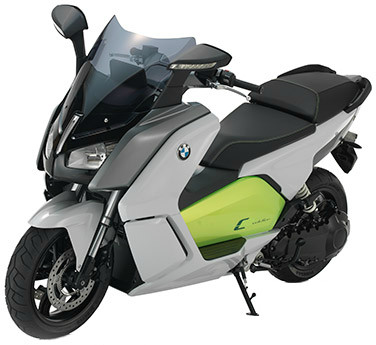
\includegraphics[width=.9\linewidth]{images/c-evolution}
}%figues de la page de garde


\def\xxpied{%
Cycle 01 -- Modéliser le comportement des systèmes multiphysiques\\
Chapitre 1 -- \xxactivite%
}

\setcounter{secnumdepth}{5}
%---------------------------------------------------------------------------

\usepackage{pgfplots}
\begin{document}
\def\pathfig{images}
%\chapterimage{png/Fond_Cin}
\pagestyle{empty}


%%%%%%%% PAGE DE GARDE COURS
\ifcours
% ==== BANDEAU DES TITRES ==== 
\begin{tikzpicture}[remember picture,overlay]
\node at (current page.north west)
{\begin{tikzpicture}[remember picture,overlay]
\node[anchor=north west,inner sep=0pt] at (0,0) {\includegraphics[width=\paperwidth]{\thechapterimage}};
\draw[anchor=west] (-2cm,-8cm) node [line width=2pt,rounded corners=15pt,draw=ocre,fill=white,fill opacity=0.6,inner sep=40pt]{\strut\makebox[22cm]{}};
\draw[anchor=west] (1cm,-8cm) node {\huge\sffamily\bfseries\color{black} %
\begin{minipage}{1cm}
\rotatebox{90}{\LARGE\sffamily\textsc{\color{ocre}\textbf{\xxnumpartie}}}
\end{minipage} \hfill
\begin{minipage}[c]{14cm}
\begin{titrepartie}
\begin{flushright}
\renewcommand{\baselinestretch}{1.1} 
\Large\sffamily\textsc{\textbf{\xxpartie}}
\renewcommand{\baselinestretch}{1} 
\end{flushright}
\end{titrepartie}
\end{minipage} \hfill
\begin{minipage}[c]{3.5cm}
{\large\sffamily\textsc{\textbf{\color{ocre} \discipline}}}
\end{minipage} 
 };
\end{tikzpicture}};
\end{tikzpicture}
% ==== FIN BANDEAU DES TITRES ==== 


% ==== ONGLET 
\begin{tikzpicture}[overlay]
\node[shape=rectangle, 
      rounded corners = .25 cm,
	  draw= ocre,
	  line width=2pt, 
	  fill = ocre!10,
	  minimum width  = 2.5cm,
	  minimum height = 3cm,] at (18.3cm,0) {};
\node at (17.7cm,0) {\rotatebox{90}{\textbf{\Large\color{ocre}{\classe}}}};
%{};
\end{tikzpicture}
% ==== FIN ONGLET 


\vspace{3.5cm}

\begin{tikzpicture}[remember picture,overlay]
\draw[anchor=west] (-2cm,-6cm) node {\huge\sffamily\bfseries\color{black} %
\begin{minipage}{2cm}
\begin{center}
\LARGE\sffamily\textsc{\color{ocre}\textbf{\xxactivite}}
\end{center}
\end{minipage} \hfill
\begin{minipage}[c]{15cm}
\begin{titrechapitre}
\renewcommand{\baselinestretch}{1.1} 
\Large\sffamily\textsc{\textbf{\xxnumchapitre}}

\Large\sffamily\textsc{\textbf{\xxchapitre}}
\vspace{.5cm}

\renewcommand{\baselinestretch}{1} 
\normalsize\normalfont
\xxcompetences
\end{titrechapitre}
\end{minipage}  };
\end{tikzpicture}
\vfill

\begin{flushright}
\begin{minipage}[c]{.3\linewidth}
\begin{center}
\xxfigures
\end{center}
\end{minipage}\hfill
\begin{minipage}[c]{.6\linewidth}
\startcontents
%\printcontents{}{1}{}
\printcontents{}{1}{}
\end{minipage}
\end{flushright}

\begin{tikzpicture}[remember picture,overlay]
\draw[anchor=west] (4.5cm,-.7cm) node {
\begin{minipage}[c]{.2\linewidth}
\begin{flushright}

\includegraphics[width=2cm]{logoCC}
\end{flushright}
\end{minipage}
\begin{minipage}[c]{.2\linewidth}
\textsl{\xxauteur} \\
\textsl{\classe}
\end{minipage}
 };
\end{tikzpicture}

\newpage
\pagestyle{fancy}

%\newpage
%\pagestyle{fancy}

\else
\fi
%% FIN PAGE DE GARDE DES COURS

%%%%%%%% PAGE DE GARDE TD
\iftd

% BANDEAU EXO
\iflivret % SI LIVRET
\begin{tikzpicture}[remember picture,overlay]
\draw[anchor=west] (-2cm,-3.3cm) node {\huge\sffamily\bfseries\color{black} %
\begin{minipage}{5cm}
\begin{center}
\LARGE\sffamily\color{ocre}\textbf{\textsc{\xxactivite}}

\begin{center}
\xxfigures
\end{center}

\end{center}
\end{minipage} \hfill
\begin{minipage}[c]{12cm}
\begin{titrechapitre}
\renewcommand{\baselinestretch}{1.1} 
\large\sffamily\textbf{\textsc{\xxtitreexo}}

\small\sffamily{\textbf{\textit{\color{black!70}\xxsourceexo}}}
\vspace{.5cm}

\renewcommand{\baselinestretch}{1} 
\normalsize\normalfont
\xxcompetences
\end{titrechapitre}
\end{minipage}};
\end{tikzpicture}
\else % ELSE NOT LIVRET
\begin{tikzpicture}[remember picture,overlay]
\draw[anchor=west] (-2cm,-4.5cm) node {\huge\sffamily\bfseries\color{black} %
\begin{minipage}{5cm}
\begin{center}
\LARGE\sffamily\color{ocre}\textbf{\textsc{\xxactivite}}

\begin{center}
\xxfigures
\end{center}

\end{center}
\end{minipage} \hfill
\begin{minipage}[c]{12cm}
\begin{titrechapitre}
\renewcommand{\baselinestretch}{1.1} 
\large\sffamily\textbf{\textsc{\xxtitreexo}}

\small\sffamily{\textbf{\textit{\color{black!70}\xxsourceexo}}}
\vspace{.5cm}

\renewcommand{\baselinestretch}{1} 
\normalsize\normalfont
\xxcompetences
\end{titrechapitre}
\end{minipage}};
\end{tikzpicture}

\fi

\else   % FIN IF TD
\fi


%%%%%%%% PAGE DE GARDE FICHE
\iffiche
\begin{tikzpicture}[remember picture,overlay]
\node at (current page.north west)
{\begin{tikzpicture}[remember picture,overlay]
\draw[anchor=west] (-2cm,-2.25cm) node [line width=2pt,rounded corners=15pt,draw=ocre,fill=white,fill opacity=0.6,inner sep=40pt]{\strut\makebox[22cm]{}};
\draw[anchor=west] (1cm,-2.25cm) node {\huge\sffamily\bfseries\color{black} %
\begin{minipage}{1cm}
\rotatebox{90}{\LARGE\sffamily\textsc{\color{ocre}\textbf{\xxnumpartie}}}
\end{minipage} \hfill
\begin{minipage}[c]{14cm}
\begin{titrepartie}
\begin{flushright}
\renewcommand{\baselinestretch}{1.1} 
\large\sffamily\textsc{\textbf{\xxpartie} \\} 

\vspace{.2cm}

\normalsize\sffamily\textsc{\textbf{\xxnumchapitre -- \xxchapitre}}
\renewcommand{\baselinestretch}{1} 
\end{flushright}
\end{titrepartie}
\end{minipage} \hfill
\begin{minipage}[c]{3.5cm}
{\large\sffamily\textsc{\textbf{\color{ocre} \discipline}}}
\end{minipage} 
 };
\end{tikzpicture}};
\end{tikzpicture}

\iflivret % SI LIVRET
\begin{tikzpicture}[overlay]
\node[shape=rectangle, 
      rounded corners = .25 cm,
	  draw= ocre,
	  line width=2pt, 
	  fill = ocre!10,
	  minimum width  = 2.5cm,
	  minimum height = 2.5cm,] at (18.5cm,.5cm) {};
\node at (17.9cm,.5cm) {\rotatebox{90}{\textsf{\textbf{\large\color{ocre}{\classe}}}}};
%{};
\end{tikzpicture}
\else  % SI PAS LIVRET
\iftd %% SI TD et PAS LIVRET
\begin{tikzpicture}[overlay]
\node[shape=rectangle, 
      rounded corners = .25 cm,
	  draw= ocre,
	  line width=2pt, 
	  fill = ocre!10,
	  minimum width  = 2.5cm,
	  minimum height = 2.5cm,] at (18.6cm,0.9cm) {};
\node at (18cm,0.9cm) {\rotatebox{90}{\textsf{\textbf{\large\color{ocre}{\classe}}}}};
%{};
\end{tikzpicture}

\else % FIN DU SI TD PAS LIVRET 
\begin{tikzpicture}[overlay]
\node[shape=rectangle, 
      rounded corners = .25 cm,
	  draw= ocre,
	  line width=2pt, 
	  fill = ocre!10,
	  minimum width  = 2.5cm,
%	  minimum height = 2.5cm,] at (18.5cm,1.1cm) {};
	  minimum height = 2.5cm,] at (18.6cm,0.5cm) {};
\node at (18cm,0.5cm) {\rotatebox{90}{\textsf{\textbf{\large\color{ocre}{\classe}}}}};
%{};
\end{tikzpicture}
\fi
\fi
\else
\fi



\vspace{8cm}
\pagestyle{fancy}
\thispagestyle{plain}

\def\columnseprulecolor{\color{ocre}}
\setlength{\columnseprule}{0.4pt} 

\def\pathfig{images}

\begin{multicols}{2}
\section*{Analyser le scooter électrique\\}


%\parpic[r]{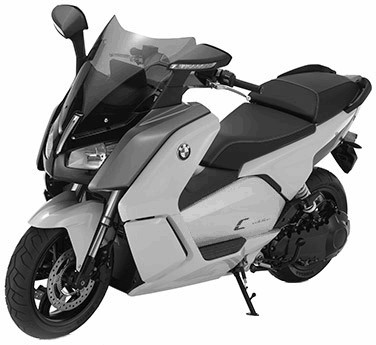
\includegraphics[width=4cm]{\pathfig/c-evolution_nb}}

Le C Évolution\textregistered ~ de BMW est le premier scooter électrique avec les mê\-mes performances qu'un scooter thermique de grosse cylindrée (\SI{600}{cm^3}). En usage urbain et péri-urbain, il offre de nombreux avantages et peu d'inconvénients. Il s'intègre facilement dans le trafic. La puissance linéaire de son moteur permet une con\-dui\-te souple, fluide et sans à-coups. Son entretien est réduit et sa consommation très économique. L'engin, silencieux et propre, est nerveux, véloce, et maniable. 
Seule ombre au tableau son prix de \num{11500} € qui peut freiner à l'achat et son bridage de vitesse à \SI{120}{km.h^{-1}} qui l'empêchera d'aller sur les autoroutes comme les scooters thermiques. 

Le schéma de la figure ci-après montre les différents éléments du scooter.



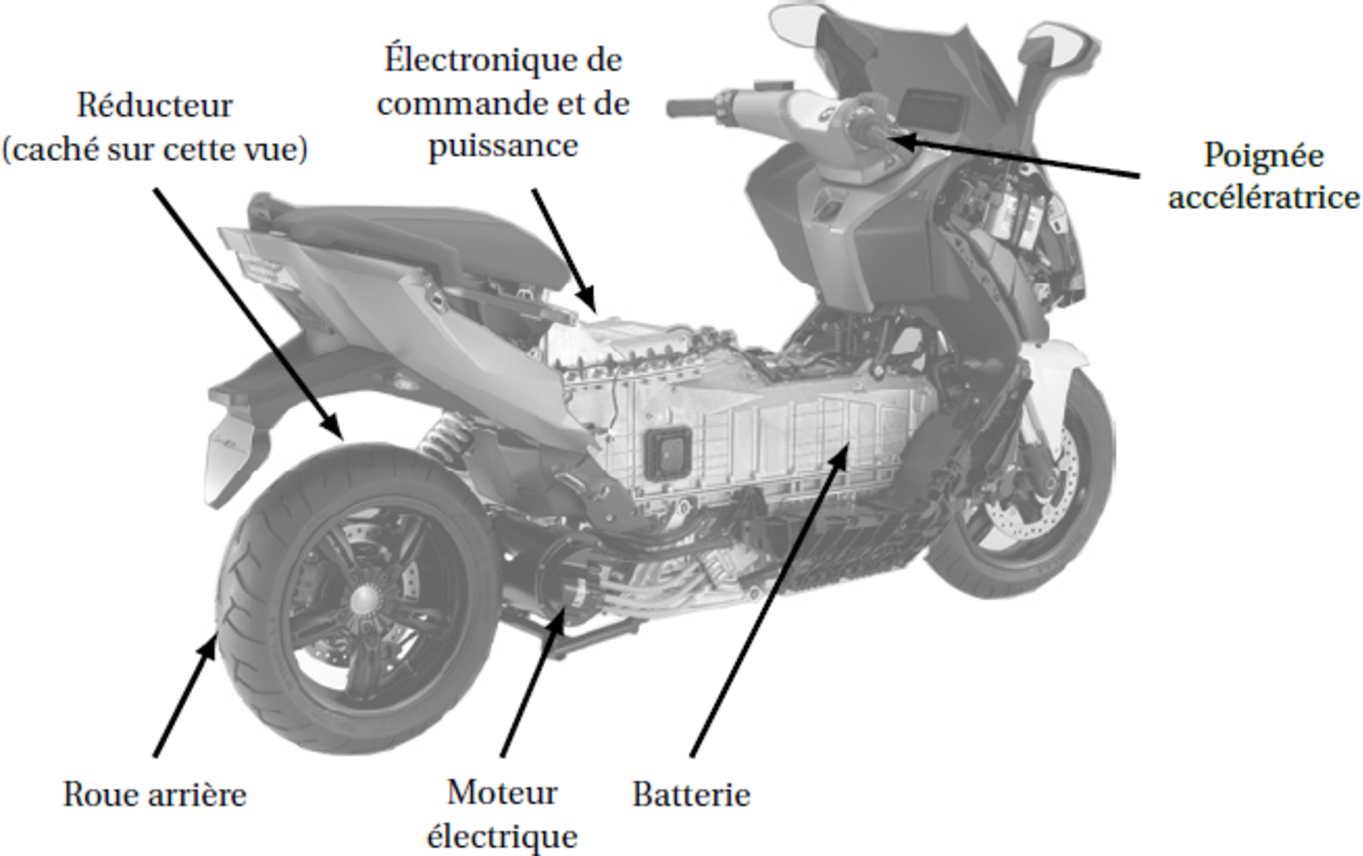
\includegraphics[width=.46\textwidth]{\pathfig/scoot_legende}
%
%\begin{figure}[!ht]
%\centering
%\scalebox{.7}{
%\begin{tikzpicture}[every node/.style={scale=.4}]
%\node[opacity=.6] at (0,0) {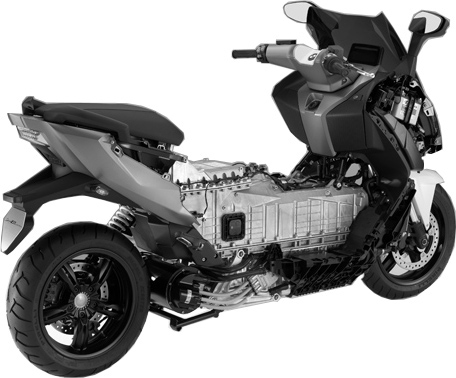
\includegraphics[width=9cm]{\pathfig/c-evolution-nu-arr_nb}};
%%\draw [gray, very thin] (-6,-5) grid [step=0.5cm] (6,5);
%%\node at (0,0) {$\circ$};
%\draw[<-,>=latex, very thick] (1.8,1.9) -- ++(2,-.3) node[right, text width=2.2cm, text badly centered]{Poignée accélératrice};
%\draw[<-,>=latex, very thick] (1.5,-.5) -- ++(-1.25,-2.5) node[below]{Batterie};
%\draw[<-,>=latex, very thick] (-.75,-1.8) -- ++(-.5,-1.2) node[below,text badly centered, text width=2cm]{Moteur électrique};
%\draw[<-,>=latex, very thick] (-2.5,-.5) -- ++(-1.5,2) node[above,align=center]{Réducteur\\(caché sur cette vue)};
%\draw[<-,>=latex, very thick] (-3.5,-2) -- ++(-.5,-1) node[below]{Roue arrière};
%\draw[<-,>=latex, very thick] (-.50,0.5) -- ++(-.5,1.) node[above, text width=3cm, text badly centered,xshift=-.3cm]{\'Electronique de commande et de puissance};
%\end{tikzpicture}}
%\caption{Architecture du scooter C Evolution\textregistered ~ de BMW. }
%\label{c_evol_archi}
%\end{figure}


\subsection*{Cahier des charges partiel}

Le cahier des charges partiel qui spécifie les principales performances annoncées par le constructeur est donné par le diagramme partiel des exigences.% (Figure \ref{c2e1exi}).



%\begin{figure}[!ht]
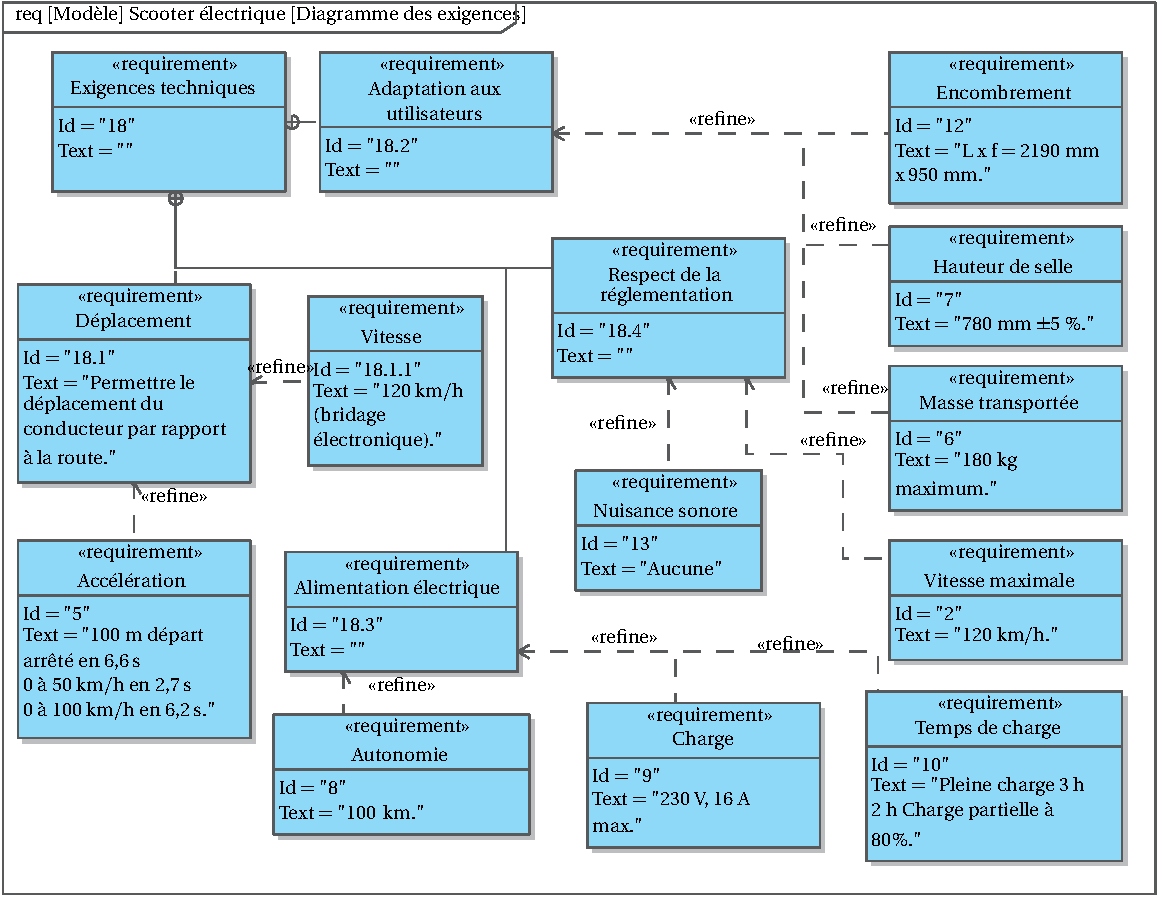
\includegraphics[width=.48\textwidth]{\pathfig/Diagramme_exigences}

%\includestandalone[width=\textwidth]{\pathfig/Diagramme_exigences}

%\caption{Diagramme partiel des exigences.}
%\label{c2e1exi}
%\end{figure}


\begin{obj}
L'objectif est de justifier le choix de la motorisation vis-à-vis du cahier des charges en utilisant un modèle de connaissance.
\end{obj}

\section*{Modéliser l'architecture du scooter électrique : schéma fonctionnel\newline}

La structure de commande du scooter électrique est simple à mettre en place à partir des composants  définis sur la figure suivante. On note l'angle de consigne $\alpha(t)$ donné au niveau de la poignée accélératrice et $v(t)$ la vitesse de déplacement du scooter (déplacement en translation). On note ${\rm pert}(t)$ les perturbations qui peuvent modifier la vitesse du scooter (elles sont ramenées au niveau du moteur).

\begin{methode}
Pour chaque composant identifier les entrées et sorties, puis relier les composants.
\end{methode}

\subparagraph{}\textit{Établir le schéma-blocs fonctionnel du scooter électrique en vous servant des indications précédentes.}


\section*{Modéliser les constituants}

Pour prévoir le comportement du scooter électrique, il est nécessaire d'élaborer un modèle de connaissance multiphysique basé sur ce schéma fonctionnel. 

Les blocs de la figure suivante représentent les différents constituants modélisés du scooter électrique. Chaque bloc représente une équation physique et nécessite donc un paramétrage précis.


%\begin{figure}[!ht]
%\centering
\begin{center}
\includegraphics[width=.98\linewidth]{\pathfig/modele_nb.png}
\textit{Constituants modélisés du scooter électrique (modèle à compléter).}
\end{center}
%\label{Scoot_02}
%\end{figure}

\begin{methode}
Afin d'éviter les erreurs, veiller à connecter des ports de même domaine fonctionnel: (triangle: signal de données, carré: électrique, rond gris: mécanique 1D en rotation).
\end{methode}




\subparagraph{}\textit{Relier les blocs de manière cohérente étant-donné l'architecture du scooter.}



\subsection*{Modèle du potentiomètre + électronique de commande et de puissance}

L'ensemble délivre une tension maximale de \SI{133}{V} pour un angle de consigne de \SI{90}{\degree} (pour \SI{0}{\degree}, l'ensemble délivre \SI{0}{V}). 


\subparagraph{}\textit{En supposant que $u_m(t)=K_1\alpha(t)$ (comportement linéaire), calculer la valeur numérique du gain $K_1$.}



\subsection*{Modèle du réducteur}
Le réducteur est constitué d'un ensemble poulies/courroie crantée et d'un réducteur de type train épicycloïdal.% (voir Figure \ref{c-evolution-reducteur}). 

\begin{center}
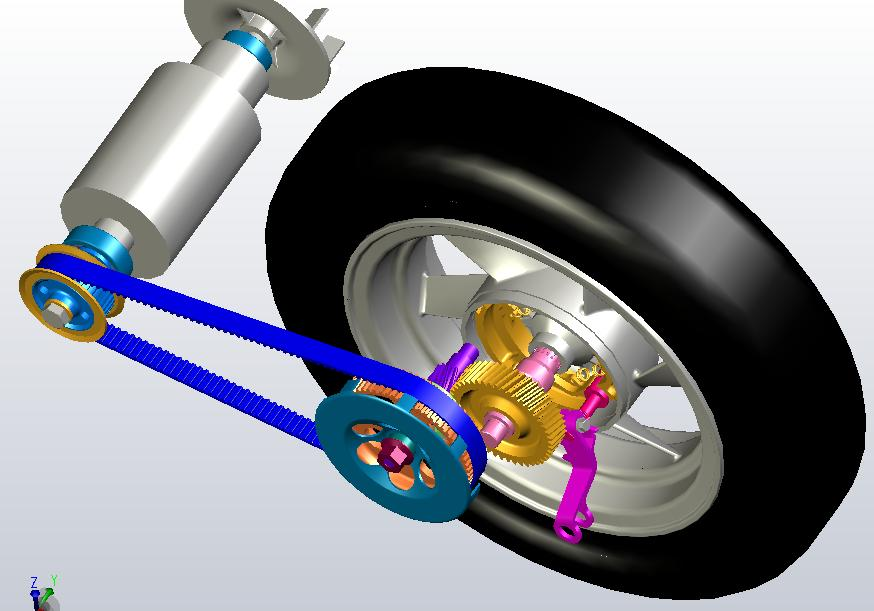
\includegraphics[width=.8\linewidth]{images/reducteur}
\end{center}
%\begin{figure}[!ht]
%\centering
%\begin{tikzpicture}[every node/.style={scale=.8},scale=.6]
%\node[opacity=.7,scale=.75] at (0,0) {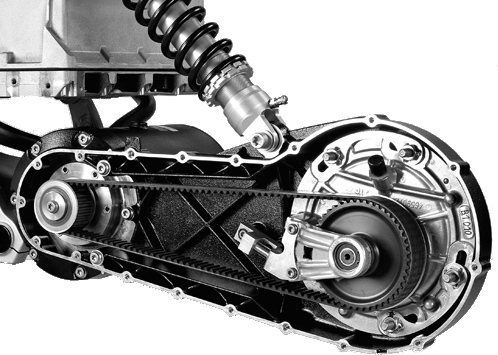
\includegraphics[width=10cm]{\pathfig/c-evolution-moteur}};
%\draw[<-,>=latex, very thick] (-4.1,-1) -- ++(-1,-1.5) node[below, text width=2cm, text badly centered]{Poulie 1 :  17 dents};
%\draw[<-,>=latex, very thick] (-1.5,-1.6) -- ++(-1,-1.5) node[below,text width=2cm, text badly centered]{Courroie crantée};
%\draw[<-,>=latex, very thick] (2.2,-2.5) -- ++(-1,-1.5) node[below,,text width=2cm, text badly centered]{Poulie 2 : 44 dents};
%\draw[<-,>=latex, very thick] (2.4,-1.) -- ++(1,3) node[above,text width=2cm, text badly centered]{Réducteur épicycloïdal à l'intérieur};
%\end{tikzpicture}
%\caption{Réducteur du scooter C Evolution\textregistered ~ de BMW.}
%\label{c-evolution-reducteur}
%\end{figure}

La poulie liée au moteur possède $Z_1=\SI{17}{dents}$ et la poulie arrière possède $Z_2=\SI{44}{dents}$. Le réducteur de type train épicycloïdal est lié d'un côté à la poulie arrière et de l'autre à la roue, de telle sorte que l'on a la relation $\dfrac{\omega_r}{\omega_p}=k_t=\num{.313}$.


On note $\theta_m(t)$ l'angle de rotation du moteur et $\omega_m(t)$ la vitesse angulaire du moteur, $\theta_r(t)$ l'angle de rotation de la roue et $\omega_r(t)$ la vitesse angulaire de la roue, $\theta_p(t)$ l'angle de rotation de la poulie arrière et $\omega_p(t)$ la vitesse angulaire de la poulie intermédiaire.

\begin{methode}
Commencer par déterminer le nombre de dents déplacées sur les $Z_2$ dents de la poulie intermédiaire lorsque le moteur fait un tour.
\end{methode}



\subparagraph{}\textit{Déterminer la constante $K_2$ telle que $\theta_r(t)=K_2\theta_m(t)$  ou $\omega_r(t)=K_2\omega_m(t)$ en fonction de $Z_{1}$, $Z_{2}$  et $k_t$. Vérifier que $K_2=\num{0.12}$.}


\subsection*{Modélisation de la roue arrière}
Le rayon $R$ de la roue en contact avec le sol est de \SI{28.65}{cm}. 

\subparagraph{}\textit{Sachant que celle-ci ne dérape pas, en déduire l'expression de $K_3$ telle que $x(t)=K_3\theta_r(t)$ ou $v(t)=K_3\omega_r(t)$.}



\subsection*{Modélisation dynamique (blocs moteur et scooter)}
Le moteur à courant continu est caractérisé par trois équations couplées :
\begin{itemize}
\item équation électrique (modélisation par circuit \textit{RL}) : $u_m(t)=e(t)+R_m\, i(t)+L_m\dfrac{\text{d}i(t)}{\text{d}t}$;
\item équations de couplage magnétique : $C_m(t)=k_c\,i(t)$ et $e(t)=k_e\,\omega_m(t)$.
\end{itemize}
On note $u_m(t)$ la tension d'alimentation, $i(t)$ le courant, $C_m(t)$ le couple fourni par le moteur, $\omega_m(t)$ la vitesse de rotation du moteur, $L_m$, $R_m$, $k_c$ et $k_e$ les constantes caractéristiques du moteur électrique.

\`A ces trois équations vient s'ajouter une équation mécanique qui caractérise la dynamique de l'ensemble des pièces en mouvement : $J_{\text{eq}}\dfrac{\text{d}\omega_m(t)}{\text{d}t}=C_m(t) - C_r(t)$  avec $C_r(t)$ couple résistant et $J_{\text{eq}}$  l'inertie équivalente.

Le moteur utilisé possède les caractéristiques suivantes :
%\begin{center}
%\noindent \begin{tabular}{|*5{c|}}
%\hline
%$R_m$&$k_e$&$k_c$&$L$&$J_{eq}$ \\ \hline
%\SI{0.02}{\ohm} & \SI{0.038}{V s} & \SI{0.038}{N  m  A^{-1}} & \SI{1e-5}{H} & \SI{0.18}{kg m^2} \\ \hline
%\end{tabular}
%\end{center}
\begin{center}
\noindent \begin{tabular}{|*5{c|}}
\hline
$R_m$&$k_e$&$k_c$&$L$&$J_{\text{eq}}$ \\ \hline
\SI{0.1}{\ohm} & \SI{0.067}{V.s} & \SI{0.067}{N.m.A^{-1}} & \SI{1e-5}{H} & \SI {0.53}{kg.m^2} \\ \hline
\end{tabular}
\end{center}


On suppose que $C_r(t)=0$ et que, compte tenu de la valeur de $L$, on néglige le terme $L_m\dfrac{\text{d}i(t)}{\text{d}t}$.


\subparagraph{}\textit{Combiner les équations précédentes simplifiées et les mettre sous la forme d'une équation différentielle du premier ordre du type $\omega_m(t) + \tau_m \frac{\text{d}\omega_m(t)}{\text{d}t}= K_m u_m (t)$. Donner les expressions du gain $K_m$ et de la constante de temps $\tau_m$.}


\subparagraph{}\textit{En combinant les relations obtenues aux différentes questions, montrer que la vitesse $v(t)$ est solution d'une équation différentielle du premier ordre de gain $K=\SI{0.76}{m.s^{-1}/\degree}$ et de constante de temps $\tau=\SI{11.8}{s}$, avec second membre dépendant de $\alpha(t)$.}


\section*{Vérification des performances du scooter électrique }

\subsection*{Vitesse maximale atteinte à plat}



On cherche dans un premier temps à vérifier que le moteur retenu permet d'atteindre la vitesse maximale à plat définie dans le cahier des charges.  On suppose qu'on accélère à fond très rapidement. L'angle $\alpha(t)$ passe instantanément de $\SI{0}{\degree}$ à  $\alpha_0=\SI{90}{\degree}$.


\subparagraph{}\textit{Indiquer quel bloc prendre dans le schéma-blocs pour modéliser l'évolution de l'angle $\alpha(t)$ parmi les blocs. Nommer cette consigne.}

%\begin{figure}[!ht]
%\centering
\begin{center}
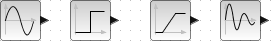
\includegraphics[width=5cm]{\pathfig/CONSIGNES_nb.png}
\textit{Consignes à choisir.}
\end{center}
%\caption{Consignes à choisir.}
%\label{Scoot_consigne}
%\end{figure}


\subparagraph{}\textit{Vérifier la performance de vitesse maximale définie dans le cahier des charges. Pour cela, on analysera l'équation différentielle en régime permanent (ou établi).}


\subsection*{Critère d'accélération}


On suppose que la vitesse du scooter est constante et égale à la vitesse maximale définie dans le cahier des charges.

\subparagraph{}\textit{Tracer l'évolution de la position du scooter au cours du temps. En combien de temps atteint-on les 100 m ?  Le cahier des charges est-il respecté ?}


Le calcul précédent est réalisé en supposant que la vitesse est constante, or compte tenu de l'équation vérifiée par la vitesse, elle ne l'est pas.

La résolution de l'équation différentielle sur la vitesse conduit à déterminer l'évolution de la vitesse en fonction du temps sous la forme : $v(t)=K\alpha_0(1-e^{-t/\tau})$. Le résultat pour une consigne d'angle de \SI{90}{\degree} est donné à la figure suivante.% Figure \ref{vitessescooter}.

%\pgfplotsset{width=7cm,compat=1.12}

%\begin{figure}[!ht]
%\centering
%\begin{tikzpicture}
%\begin{axis}[xlabel={Temps (s)}, ylabel={Vitesse ($\SI{}{m. s^{-1}}$)},xmin=0,xmax=50,ymin=0,grid=major,width=8cm,height=4cm,minor y tick num=4,minor x tick num=1,font=\small ]
%\addplot[cyan,domain=0:50,samples=201,thick]{.76*90*(1-exp(-x /11.8))};
%\end{axis}
%\end{tikzpicture}
%\caption{\'Evolution de la vitesse du scooter au cours du temps.}
%\label{vitessescooter}
%\end{figure}


\begin{center}
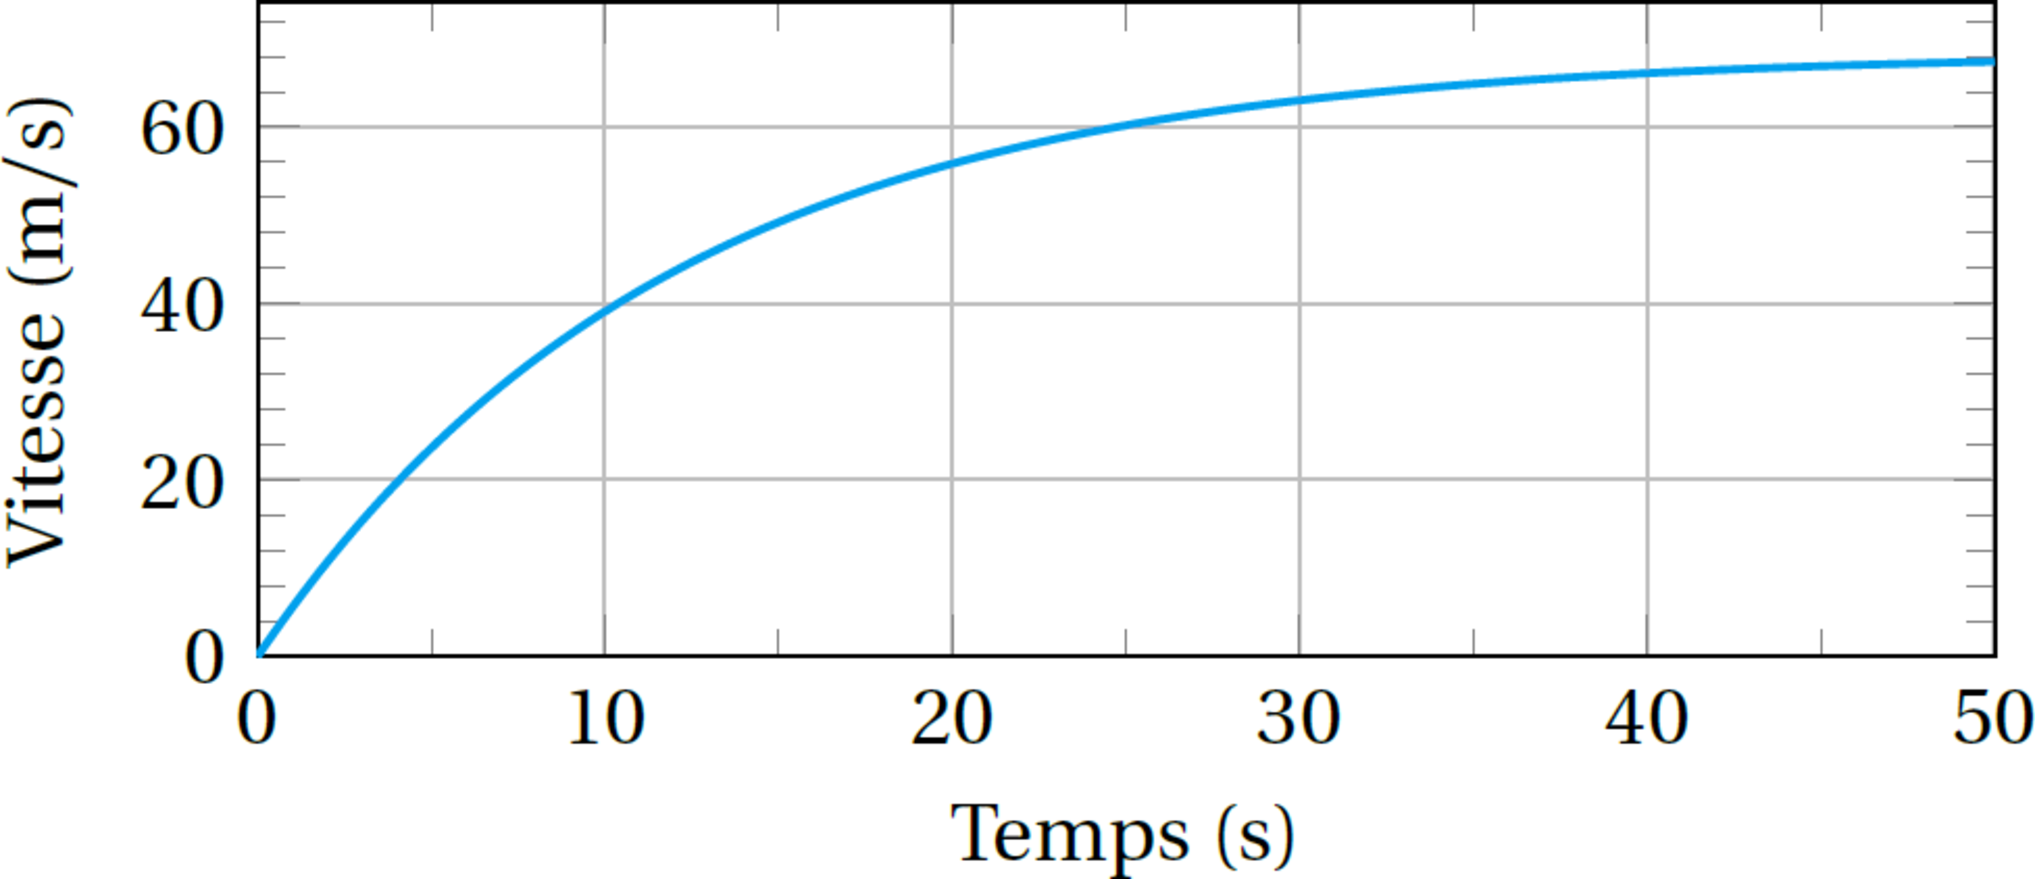
\includegraphics[width=\linewidth]{vitesse}
\textit{\'Evolution de la vitesse du scooter au cours du temps.}
\end{center}

\subparagraph{}\textit{En combien de temps peut-on considérer que la vitesse maximale est atteinte à $5 \%$ près ? Conclure sur l'hypothèse de vitesse constante.}





Le modèle multiphysique mis en place permet de réaliser une simulation de la position du scooter au cours du temps (voir figure suivante).%Figure \ref{c-evolution_simulation}). 
%
%\begin{figure}[!ht]
%\centering
%%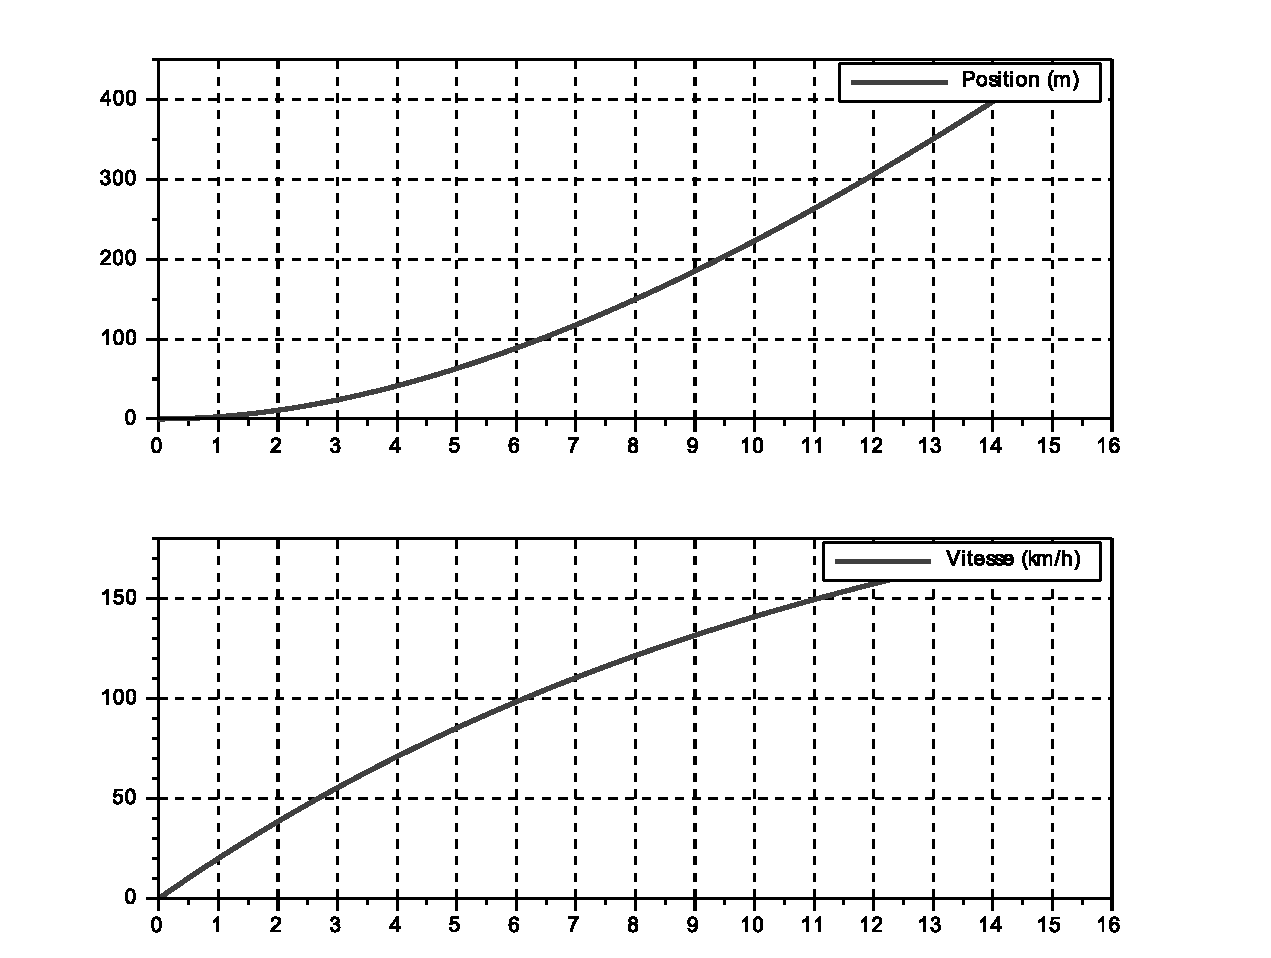
\includegraphics[width=10cm]{\pathfig/c-evolution_simulation}
%%\includestandalone{\pathfig/c-evolution_simulation_01}
%%\includestandalone{\pathfig/c-evolution_simulation_02}
%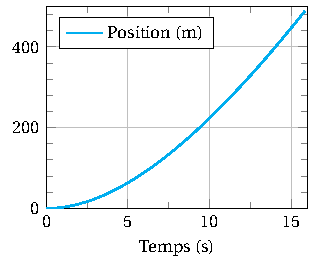
\includegraphics[width=10cm]{\pathfig/c-evolution_simulation_01}
%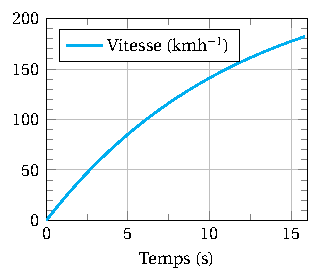
\includegraphics[width=10cm]{\pathfig/c-evolution_simulation_02}
%\caption{\'Evolution de la position et de la vitesse du scooter C Evolution\textregistered ~ de BMW obtenue par le modèle.}
%\label{c-evolution_simulation}
%\end{figure}
%


\begin{center}
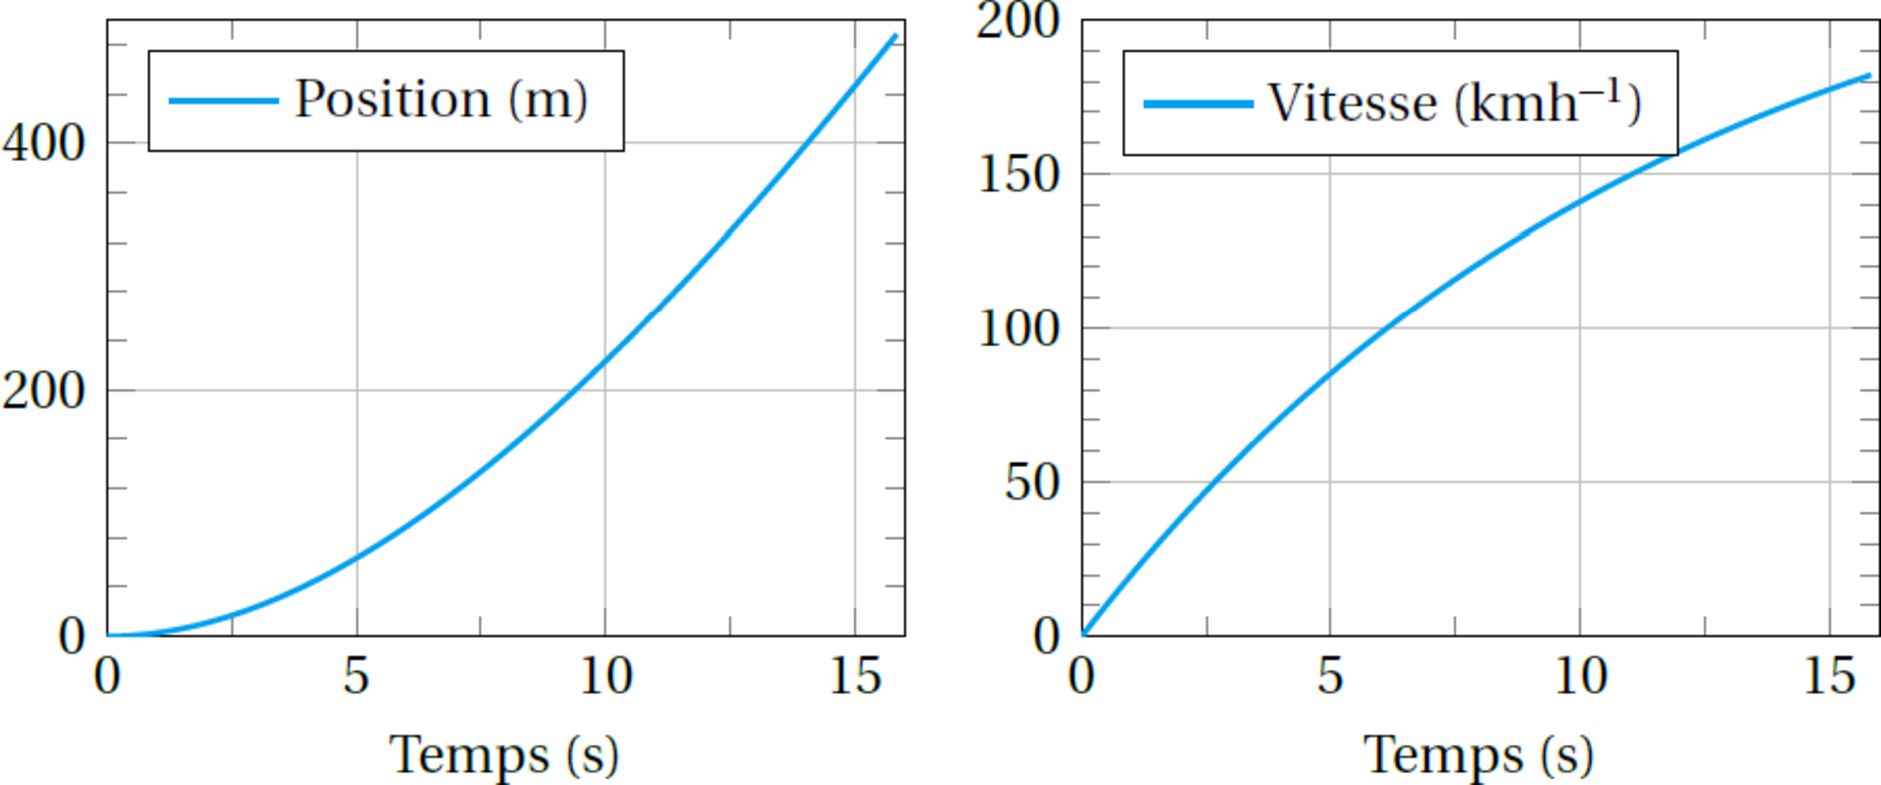
\includegraphics[width=\linewidth]{vitesse_2}
\textit{\'Evolution de la position et de la vitesse du scooter C Evolution\textregistered ~ de BMW obtenue par le modèle.}
\end{center}
\section*{Retour sur le cahier des charges}

\subparagraph{}\textit{Indiquer en combien de temps les \SI{100}{m} seront atteints. Compléter le diagramme de synthèse de l'étude. Conclure quant au respect du cahier des charges. Quelles hypothèses du modèle mis en place doit-on remettre en cause pour se rapprocher de la réalité ?}


%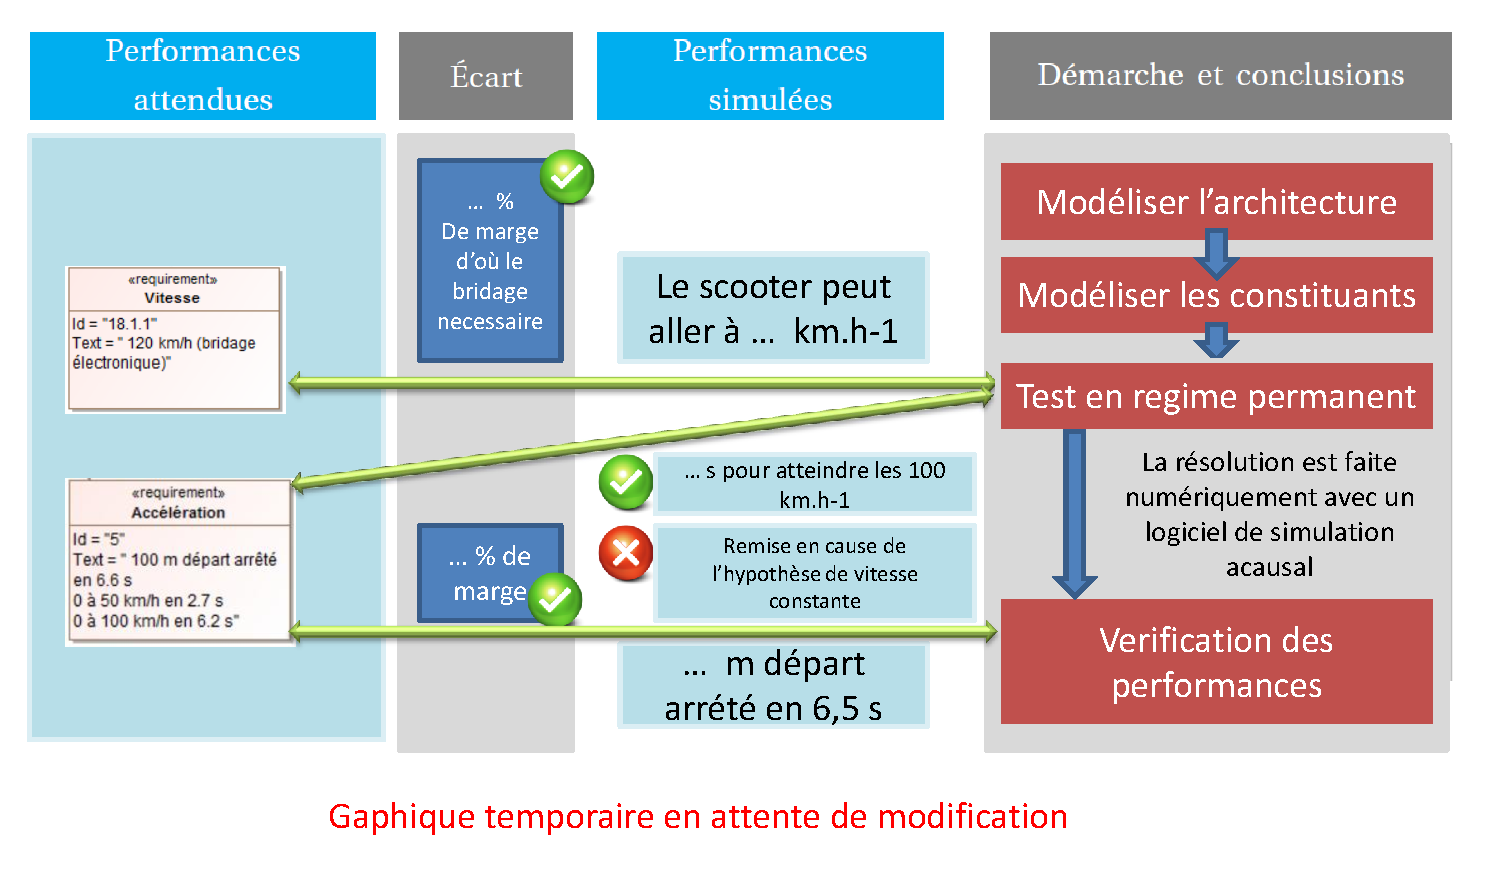
\includegraphics[width=.9\textwidth]{CHAP2/ex_ScootElec/images/Bilan}


%{\centering\includestandalone[width=.9\textwidth]{\pathfig/image_bilan}\par}

%\end{conclusion}

%\begin{remarque}
%Les développements que l'on fera en SI permettront d'affiner les modèles et ainsi justifier au mieux le cahier des charges.
%\end{remarque}


\end{multicols}
{\centering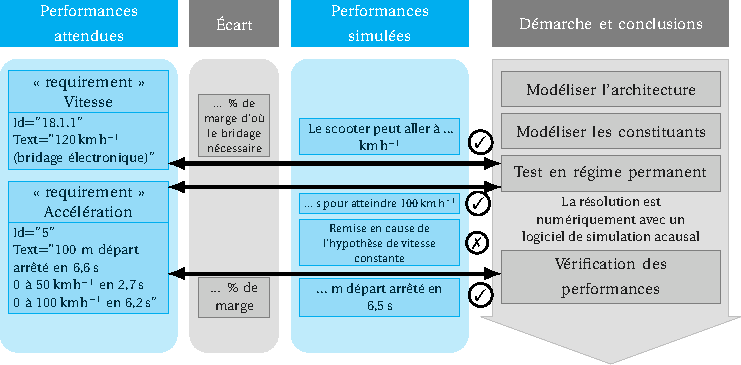
\includegraphics[width=.9\textwidth]{\pathfig/image_bilan}\par}
\end{document}

\end{exoGuide}

\begin{correction}

\def\pathfig{CHAP2/ex_ScootElec/images}
\begin{questions}
\item ~

\begin{center}
\scalebox{.8}{
\begin{tikzpicture}[scale=.8,every nodes/.style={scale=.8}]
\sbEntree{a};
\sbBloc[3]{u}{Poignée}{a};
\sbRelier[$\alpha(t)$]{a}{u};
\sbBlocL[3]{mm}{Carte commande}{u};
\sbBloc[3]{m}{Moteur}{mm};
\sbRelier[$u(t)$]{mm}{m};
\sbBloc[3]{r}{Réducteur}{m};
\sbRelier[$\omega_m(t)$]{m}{r};
\sbBloc[3]{v}{Roue}{r};
\sbRelier[$\omega_r(t)$]{r}{v};
\sbSortie[3]{vv}{v};
\sbRelier[$v(t)$]{v}{vv};
\sbDecaleNoeudy[-4]{m}{mm}
\sbRelier[Pert$(t)$]{mm}{m}
\end{tikzpicture}}
\end{center}

\item ~

\begin{center}
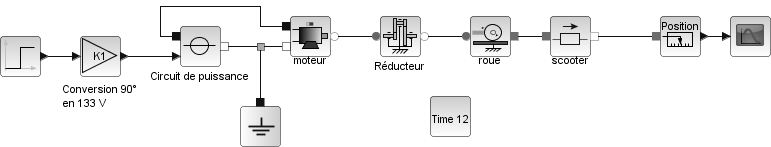
\includegraphics[width=11cm]{\pathfig/Corrige_nb.png}
\end{center}


\item Sachant que le comportement est supposé linéaire, comme on a $u(t)=\SI{133}{V}$ quand $\alpha(t)=\SI{90}{\degree}$, on en déduit que $u(t)=\dfrac{133}{90}\alpha(t)$.

On en déduit ainsi que $K_1=\dfrac{133}{90}=\num{1.48}$ (en \si{V/\degree}).

\item Le rapport de réduction du système poulie-courroie est tel que : $\dfrac{\omega_p}{\omega_m} = \dfrac{Z_1}{Z_{2}}$. En effet, lorsque le moteur fait un tour, il déplace $Z_{1}$ dents sur les $Z_2$ dents de la poulie intermédiaire qui a donc tourné de $\dfrac{Z_1}{Z_{2}}$ tour.
De plus, $\dfrac{\omega_r}{\omega_p}=k_t$.
D'où $\dfrac{\omega_r(t)}{\omega_m(t)}=\dfrac{Z_1}{Z_{2}}\times k_t=\dfrac{17}{44}\times \num{.313} =\num{0.12}$.


\item Si l'on suppose que la roue ne glisse pas sur le sol, alors en notant $x(t)$ le déplacement du scooter et $\theta_r(t)$ l'angle de rotation de la roue, on a la relation : $x(t) = R \theta_r(t)$ (avec $\theta_r$ en radian). Lorsque la roue tourne d'un tour (donc de $2\pi$ radians), la roue a avancé de la valeur du périmètre soit $2\pi R$. En dérivant cette relation, on obtient : $v(t)=\dot x(t) = R \dot \theta_r(t) = R\omega_r(t)$. Ainsi, $K_3=R$.

\item L'objectif est de ne garder que $u_m(t)$ et $\omega_m(t)$ comme variable dépendant du temps. L'équation de dynamique devient :  $J_{\text{eq}}\dfrac{\d\omega_m(t)}{\text{d}t}=C_m(t)$. En remplaçant $C_m(t)$ par $k_c\,i(t)$, on obtient : $J_{\text{eq}}\dfrac{\d\omega_m(t)}{\text{d}t}=k_c\, i(t)$ soit $i(t) = \dfrac{J_{\text{eq}}}{k_c} \dfrac{\d\omega_m(t)}{\text{d}t}$. L'équation électrique devient : $u_m(t)=e(t)+R_m\, i(t)$ et en remplaçant $e(t)=k_e\,\omega_m(t)$, on obtient :  $u_m(t)=k_e\,\omega_m(t)+R_m\, i(t)$. En remplaçant $i(t)$ dans l'équation électrique, on obtient : 
$u_m(t)=k_e\,\omega_m(t)+R_m\,\dfrac{J_{\text{eq}}}{k_c} \dfrac{\d\omega_m(t)}{\text{d}t}$ ce qui correspond bien à une équation différentielle du premier ordre.

Cette équation peut s'écrire sous la forme générique d'une équation différentielle du premier ordre : $\tau_m \dfrac{\d\omega_m(t)}{\text{d}t} + \omega_m(t)= K_m u_m(t)$. Soit en divisant toute l'équation différentielle par $k_e$, 
$\dfrac{u_m(t)}{k_e} =\omega_m(t)+ \dfrac{R_m\,J_{\text{eq}}}{k_e k_c} \dfrac{\d\omega_m(t)}{\text{d}t}$. Ainsi, $K_m= \dfrac{1}{k_e}$ et $\tau_m=\dfrac{R_m\,J_{\text{eq}}}{k_e k_c}$.

\item Sachant que $v(t)=K_3 \omega_r (t)$ et $\omega_r(t)=K_2\omega_m(t)$, puis que $u_m(t)=K_1 \alpha (t)$, on obtient directement en remplaçant $\omega_m(t)$ par $\dfrac{v(t)}{K_3 K_2}$, $\dfrac{K_1}{k_e} \alpha(t) =\dfrac{v(t)}{K_3 K_2}+ \dfrac{R_m\,J_{\text{eq}}}{k_e k_c K_3 K_2} \dfrac{\text{d}v(t)}{\text{d}t}$.

En multipliant l'équation par $K_3 K_2$, le nouveau gain est $K=\dfrac{K_1 K_2 K_3}{k_e}$ et la constante de temps est toujours la même $\tau=\tau_m$. En effectuant les applications numériques, on obtient bien les valeurs demandées.

\item Il faut retenir le deuxième bloc qui correspond à un échelon.

\item En régime permanent, la dérivée est nulle, la vitesse vaut donc $K \alpha_0$ soit $\num{0.76} \times 90 = \SI{68.4}{m.s^{-1}}$ ou $\SI{246}{km. h^{-1}}$. On dépasse très largement les $\SI{120}{km. h^{-1}}$ autorisés ce qui n'est pas correct vis-à-vis de la législation: cela justifie le bridage électronique du scooter !

\item Si la vitesse est constante, on obtient une position égale à une droite passant par l'origine (la position est l'intégrale de la vitesse). Ainsi $x(t)=v_{\text{max}}\times t$. On atteint ainsi \SI{100}{m} en $100/\num{33.3}=\SI{3}{s}$ ce qui est beaucoup moins que ce qu'indique le cahier des charges. Ceci est normal car on ne peut pas négliger le temps du passage de 0 à $\SI{120}{km. h^{-1}}$.

\item On peut considérer que la vitesse maximale est atteinte à $5 \%$ près au bout de $3\tau$ soit $\SI{36}{s}$. On en déduit que l'hypothèse de vitesse constante est totalement fausse. On n'atteindra pas les 100 m en 3 s mais en beaucoup plus.


\item On atteint les 100 m en \SI{6.5}{s} ce qui correspond à la valeur annoncée dans le cahier des charges. On a cependant omis de prendre en compte les frottements et la résistance à l'air, ce qui ralentira plus le scooter. Qui plus est, la consigne en échelon n'est pas nécessairement réaliste car on ne passe pas immédiatement de 0 à \SI{90}{\degree}.

Pour améliorer le modèle, il faudrait également réaliser un asservissement pour limiter la vitesse à $\SI{120}{km. h^{-1}}$ avec un bloc de contrôle de la tension d'alimentation envoyée au moteur.

%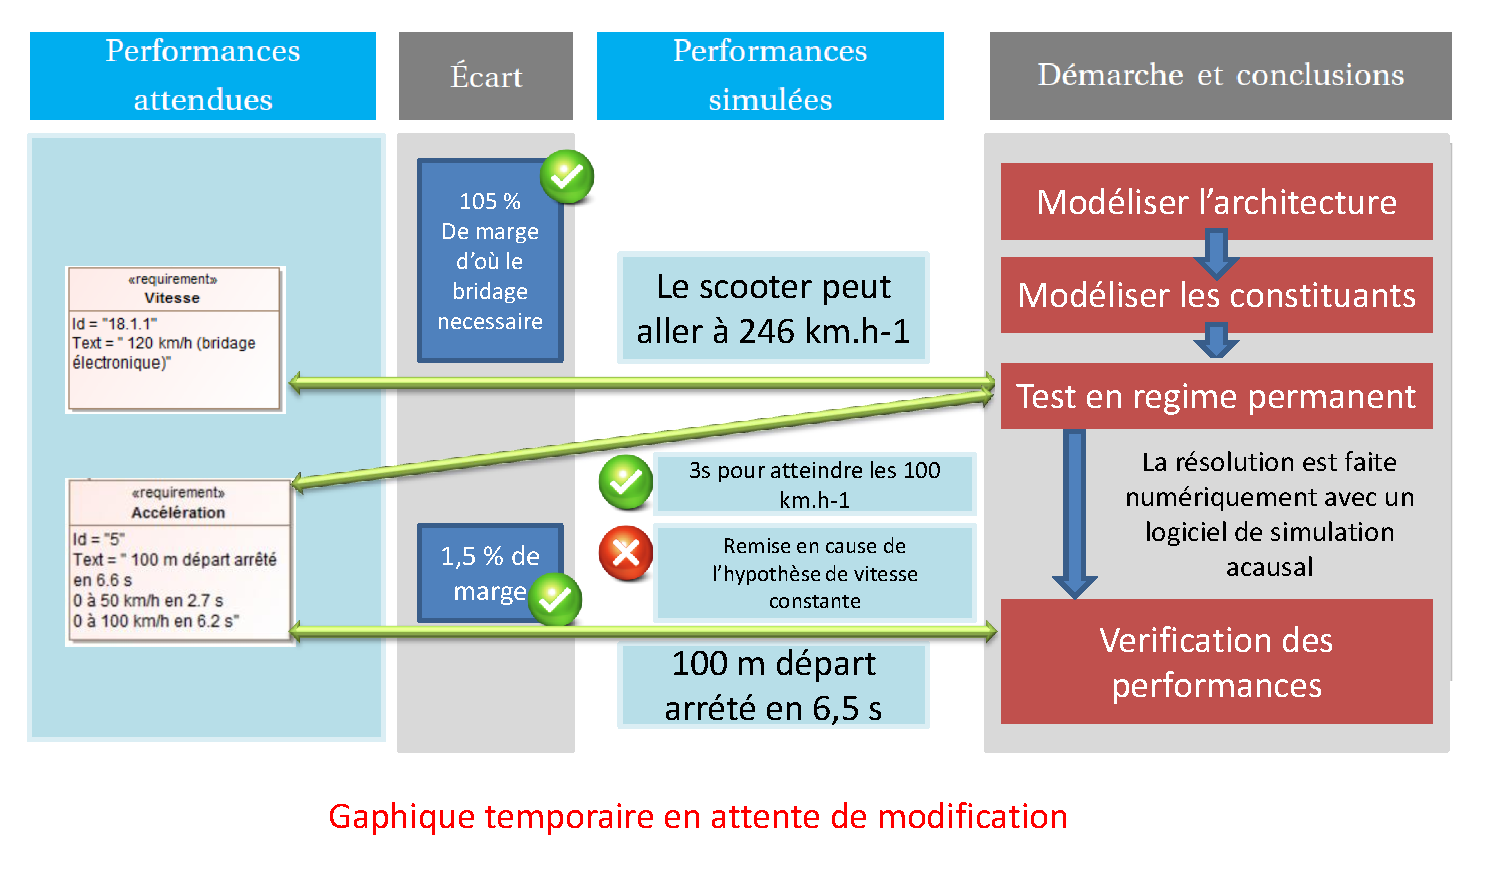
\includegraphics[width=.9\textwidth]{CHAP2/ex_ScootElec/images/BilanCorr}

{\centering\includestandalone[width=.9\textwidth]{\pathfig/image_bilan_corr}\par}


\end{multicols}



\end{document}